\documentclass[aspectratio=169]{beamer}
\usetheme{default}
\usepackage{minted}
\usepackage{xcolor}
\usepackage{tcolorbox}
\usepackage{graphicx} 
\usepackage[font=Times, timeinterval=1, timeduration=15]{tdclock}
\usepackage{fontspec}
\usepackage{pifont}
\usepackage{hyperref}

% Définir la police principale
% \setmainfont{Clear Sans Light}

\setbeamertemplate{footline}[frame number]
\setbeamertemplate{navigation symbols}{}

%\setbeamertemplate{background}{\rule{0em}{.99\paperheight}\hspace{.5em}{\color{black}\tiny\bfseries\crono}}

\BeforeBeginEnvironment{minted}{\begin{tcolorbox}}%
\AfterEndEnvironment{minted}{\end{tcolorbox}}%

\AtBeginSection[]{
   \begin{frame}
   \begin{center}{\Large Plan }\end{center}
   \tableofcontents[currentsection,hideothersubsections]
   \end{frame} 
}

\AtBeginSubsection[]{
    \begin{frame}
    \begin{center}{\Large Plan }\end{center}
    \tableofcontents[currentsection, currentsubsection]
    \end{frame}
}

\hypersetup{
    colorlinks=true,
    linkcolor=blue,
    urlcolor=cyan
}

% Item style

\setbeamertemplate{itemize item}{\ding{108}}

% Block style

\setbeamercolor{block body alerted}{fg=white,bg=red}
\setbeamercolor{block body standard}{fg=black,bg=white}
\setbeamertemplate{blocks}[rounded][shadow=false]

% Alias for highlight text in orange and bold
\newcommand{\highlight}[1]{\textcolor{orange}{\textbf{#1}}}

%Information to be included in the title page:
\title{Kokkos and performance portability: an introduction for all}
\author{Mathieu Lobet and the CExA team}
\institute{CEA}
\date{2024}

\begin{document}

\frame{

% _____________________________________________________________________________

\titlepage

% \begin{center}
%     
\includegraphics[width=0.3\textwidth]{../../images/cexa_logo.png}
% \end{center}

\begin{center}
    \begin{minipage}{0.3\textwidth}
        \centering
        
\includegraphics[width=0.8\textwidth]{../../images/kokkos.png}
    \end{minipage}%
    \begin{minipage}{0.3\textwidth}
        \centering
        
\includegraphics[width=0.8\textwidth]{../../images/cexa_logo.png}
    \end{minipage}
\end{center}

}

% _____________________________________________________________________________

\section{Introduction}

% \begin{frame}
%     \initclock
%     \centering
%     \Huge Introduction
% \end{frame}

% _____________________________________________________________________________

\begin{frame}
    \frametitle{This course is open-source}
    
    \begin{center}

    
\includegraphics[width=0.3\textwidth]{../../images/GitHub-logo.png}

    \href{https://github.com/CExA-project/cexa-kokkos-tutorials}{https://github.com/CExA-project/cexa-kokkos-tutorials}

    \end{center}
    
\end{frame}

% _____________________________________________________________________________

\begin{frame}
\frametitle{Prerequisite}

This course is intended for beginners in Kokkos and performance portability without strong C++ knowledge. 

\begin{itemize}
    \item Basic knowledge of C/C++
    \item Basic knowledge of parallel programming
    \item Basic knowledge of CMake
    \item Basic knowledge of a Linux environment
\end{itemize}

\end{frame}

% _____________________________________________________________________________

\begin{frame}
    \frametitle{Duration of the course}
    
    \begin{itemize}
        \item Course + practical work: full day 
        \item Course + corrected exercise: half day
        \item Short version: 3 hours
    \end{itemize}
    
 \end{frame}

% _____________________________________________________________________________

\begin{frame}
\frametitle{Presentation of CExA}

\begin{center}
    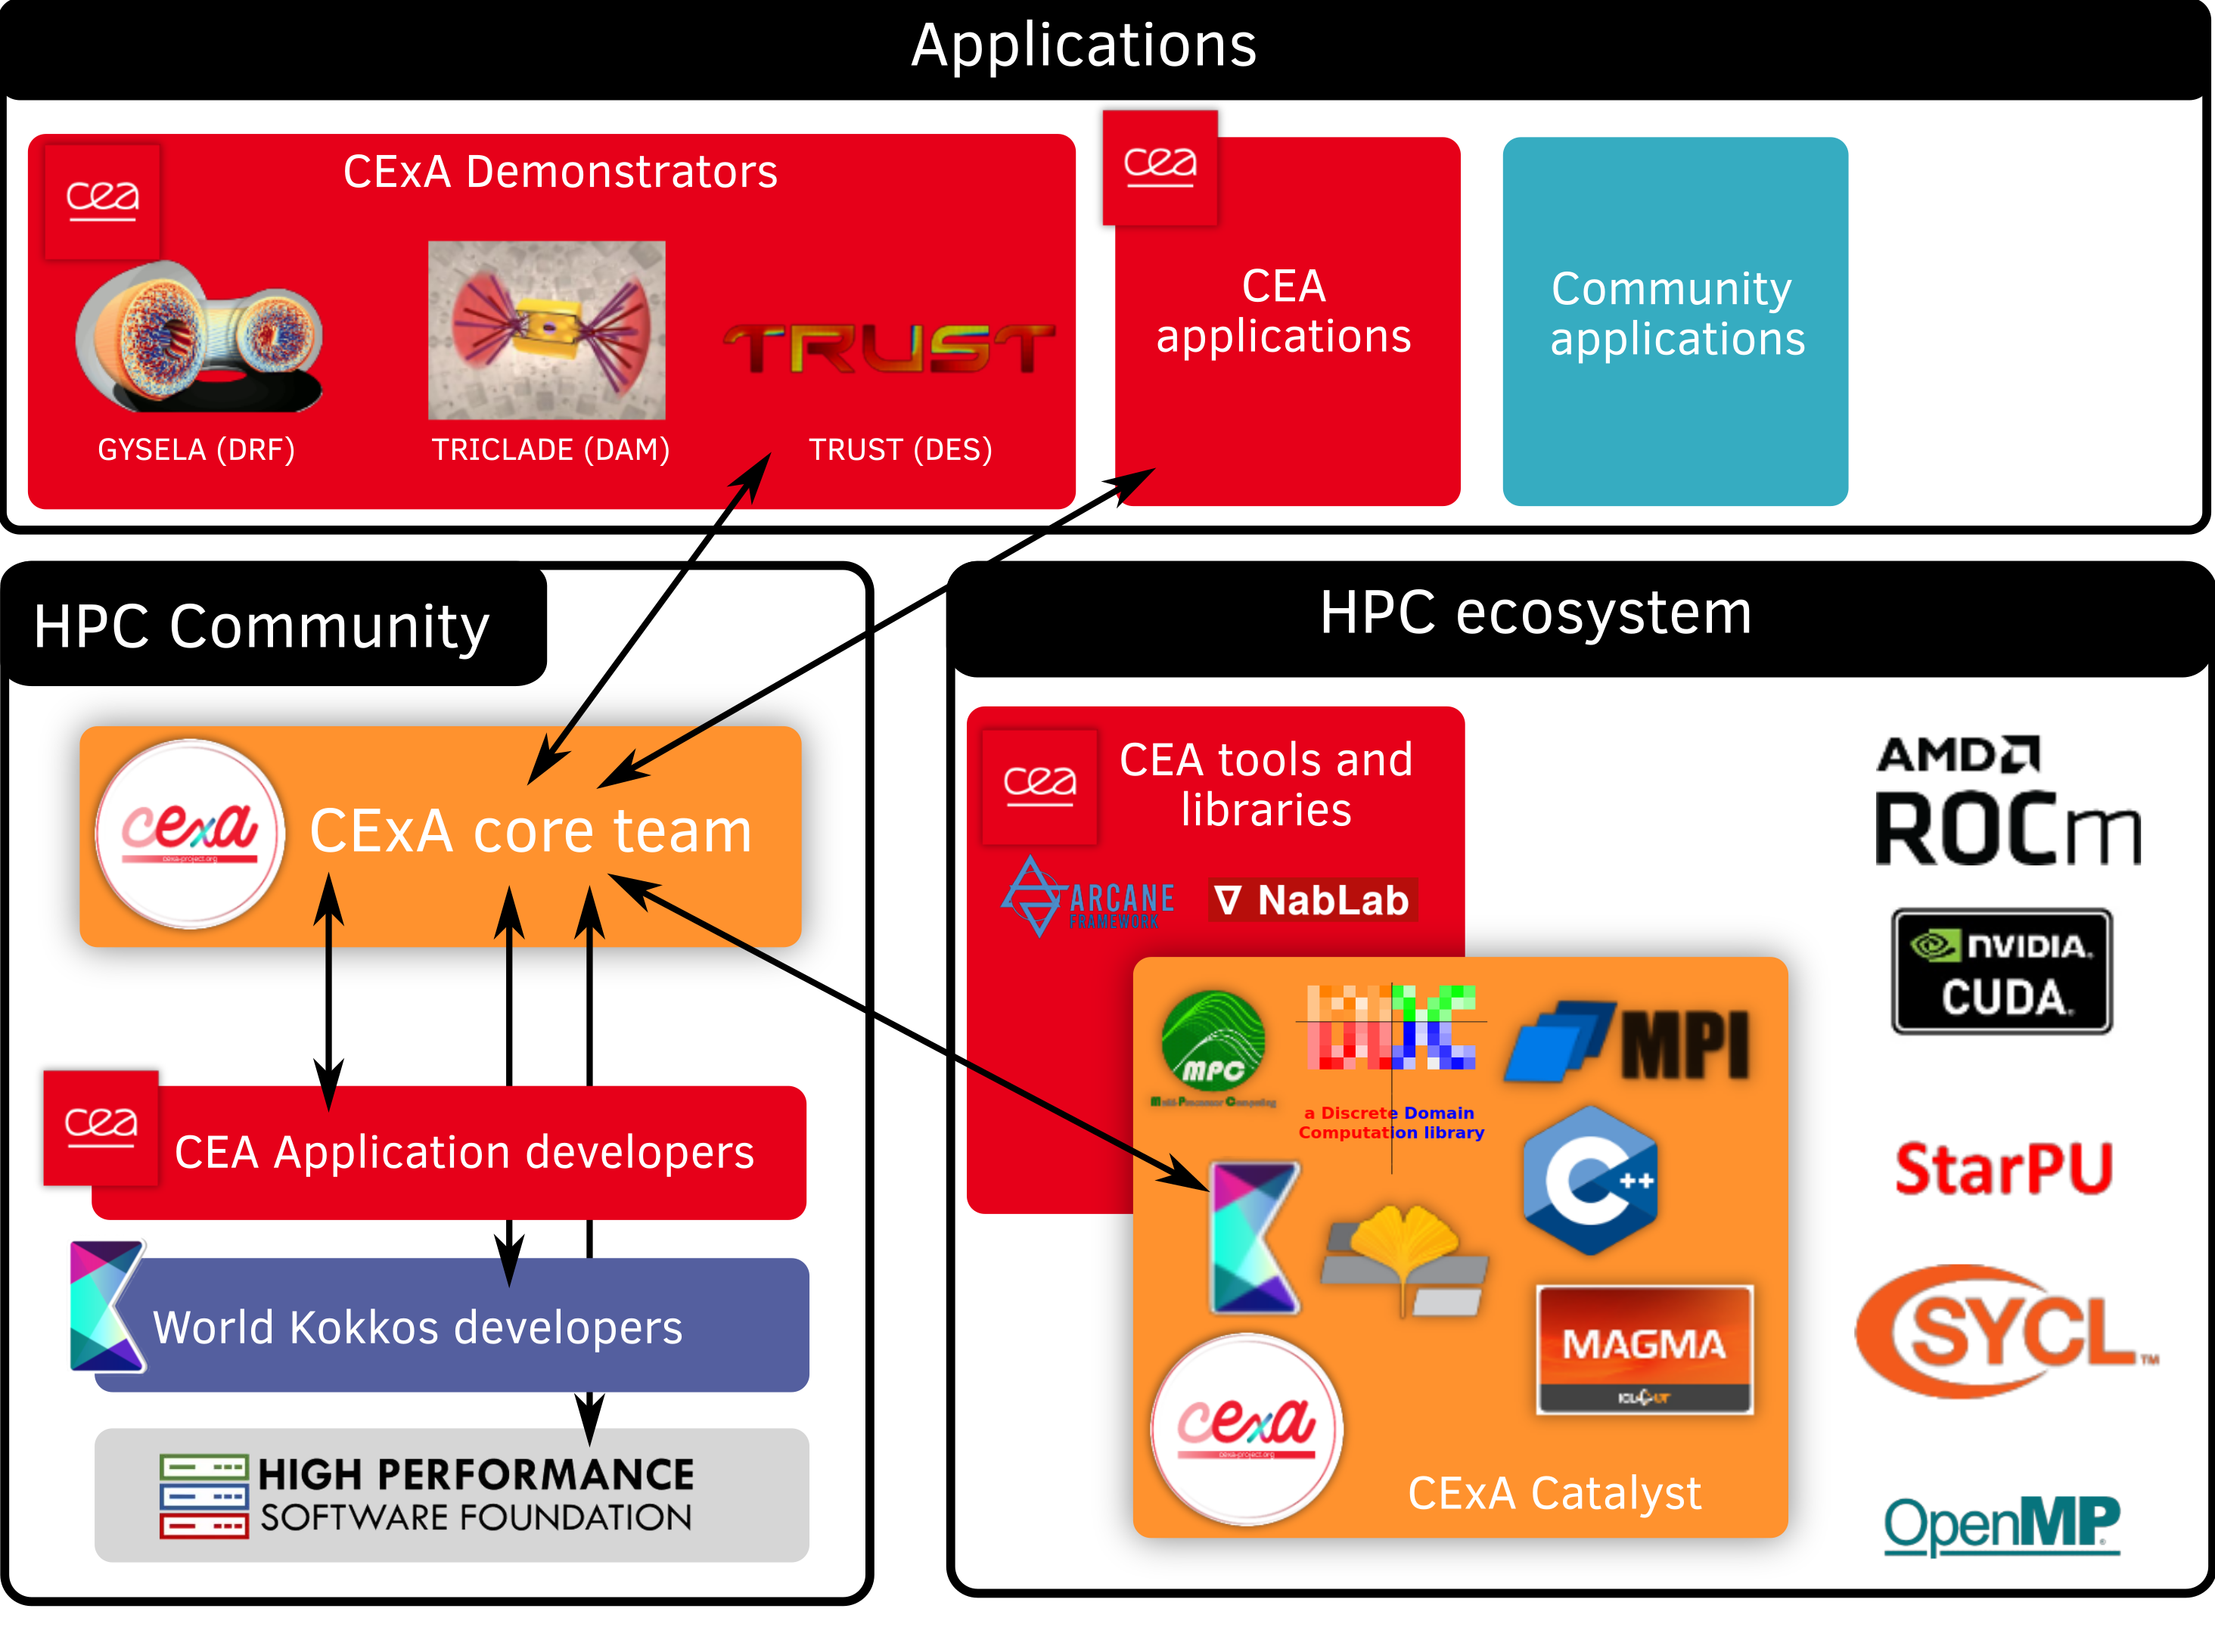
\includegraphics[width=0.7\textwidth]{../../images/cexa.png}
\end{center}

\end{frame}

% _____________________________________________________________________________

\begin{frame}
\frametitle{Current supercomputers use a wide variety of hardware technologies}

\begin{figure}
\begin{center}
    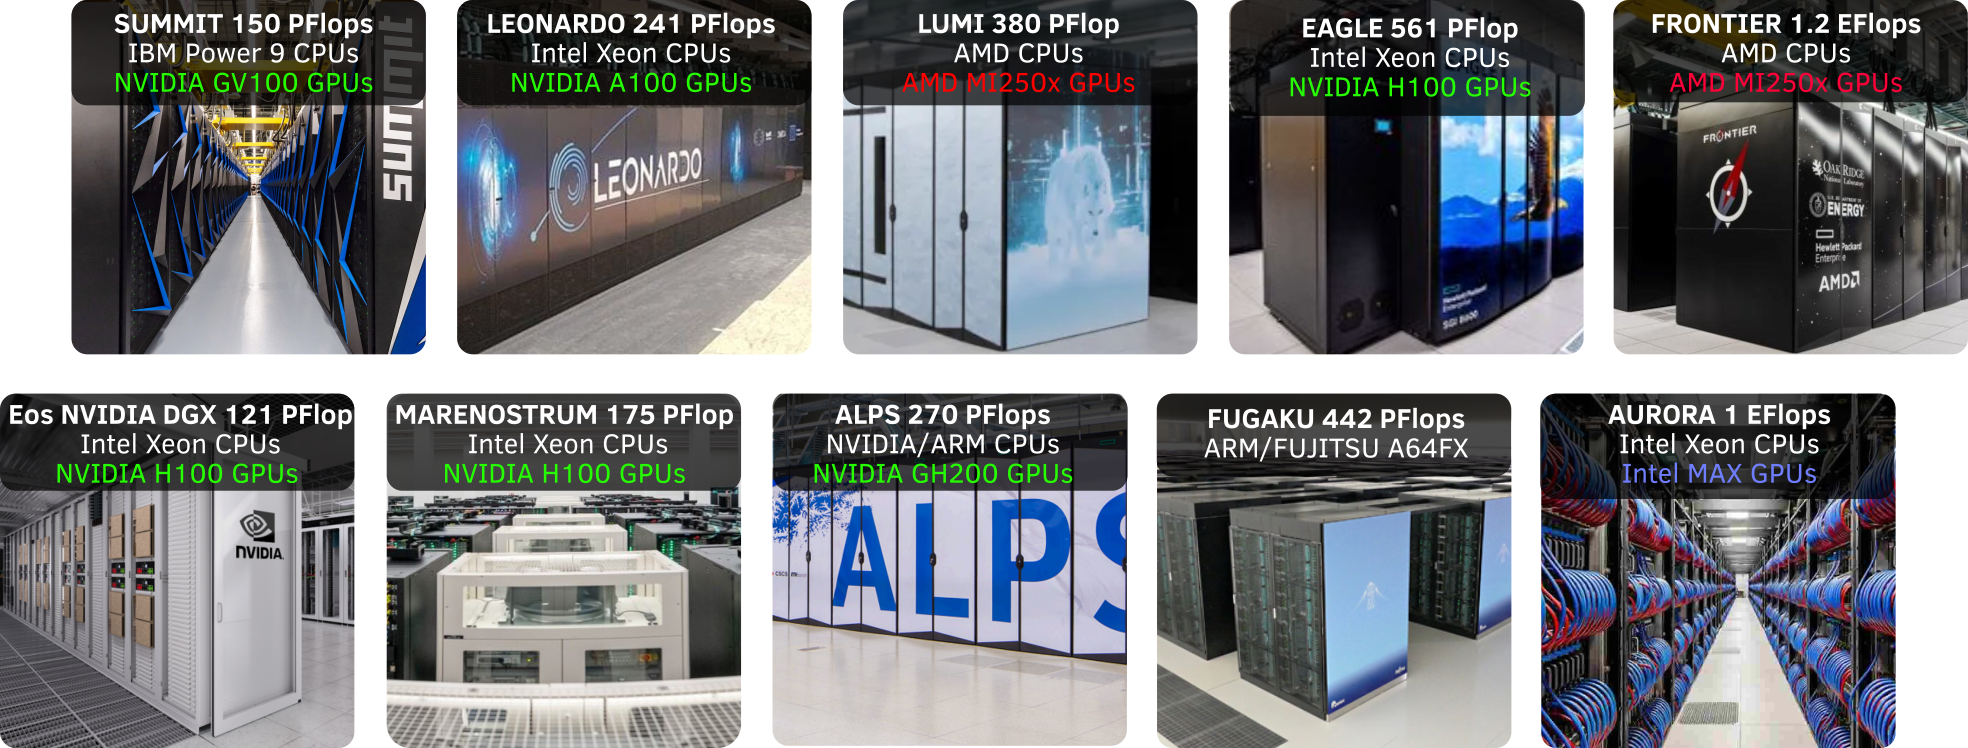
\includegraphics[width=1\textwidth]{../../images/top10_super_computers.png}
    \caption{Top 10 supercomputers in the world in June 2024}
\end{center}
\end{figure}

\begin{itemize}
\item Heterogeneous nodes: mix of CPU and GPU accelerators
\item Many CPU (Intel, AMD, ARM, RISC) and GPU vendors (NVIDIA, AMD, Intel)
\end{itemize}

\end{frame}

% _____________________________________________________________________________

\begin{frame}
\frametitle{EuroHPC supercomputers}

\begin{figure}
\begin{center}
    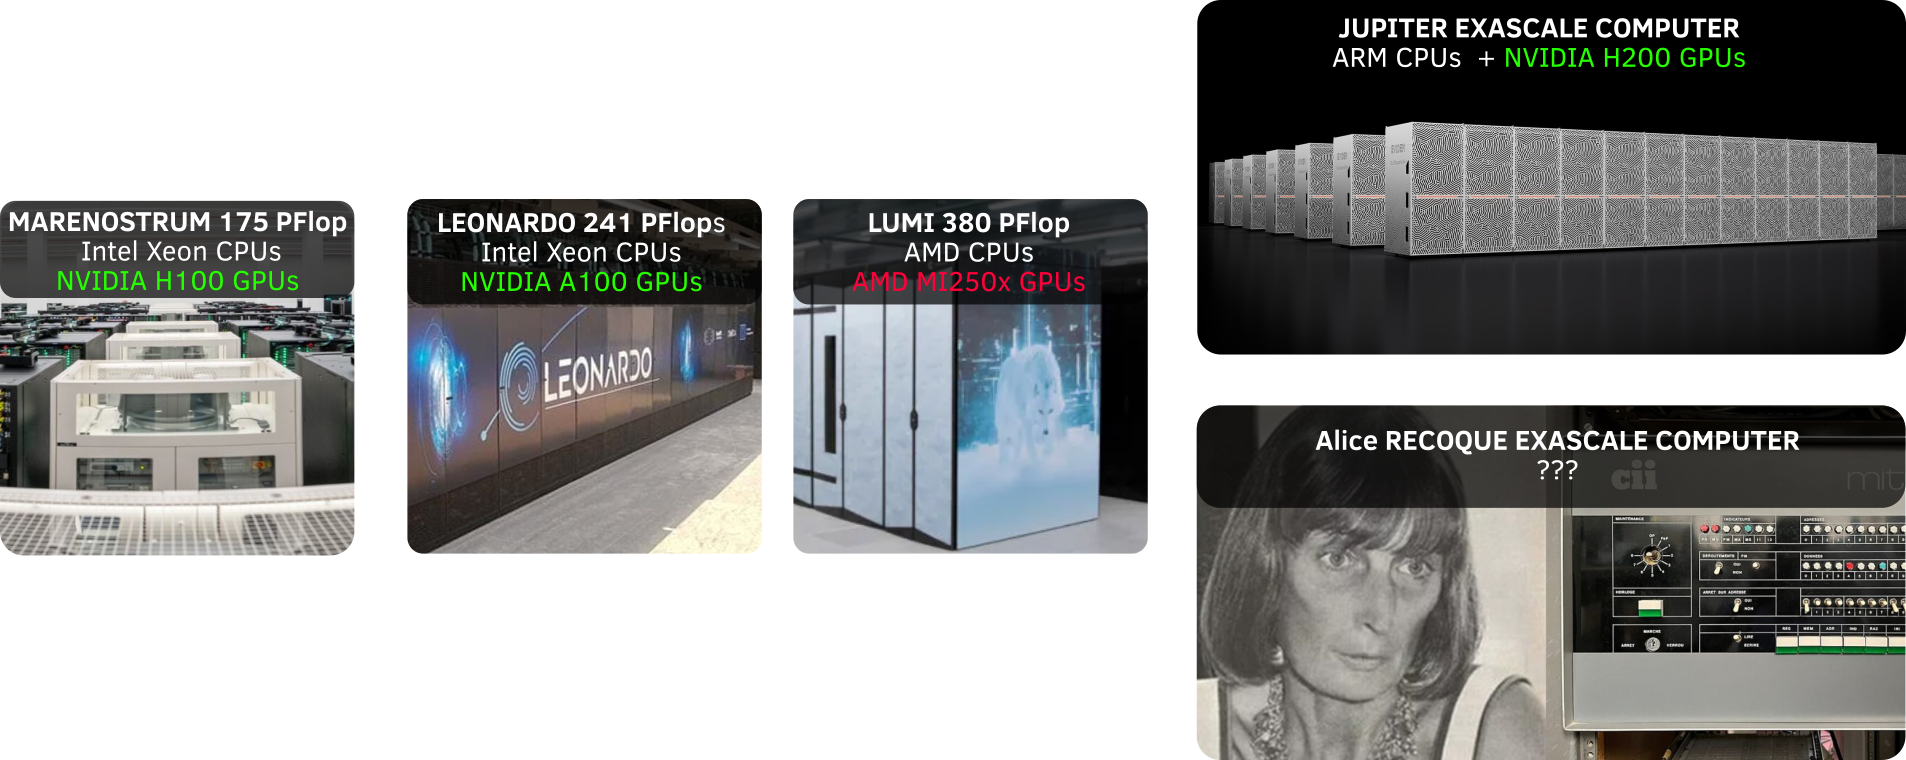
\includegraphics[width=1\textwidth]{../../images/euroHPC.png}
    \caption{EuroHPC supercomputers}
\end{center}
\end{figure}

\end{frame}

% _____________________________________________________________________________

\begin{frame}
\frametitle{National academic supercomputers}

\begin{figure}
    \begin{center}
    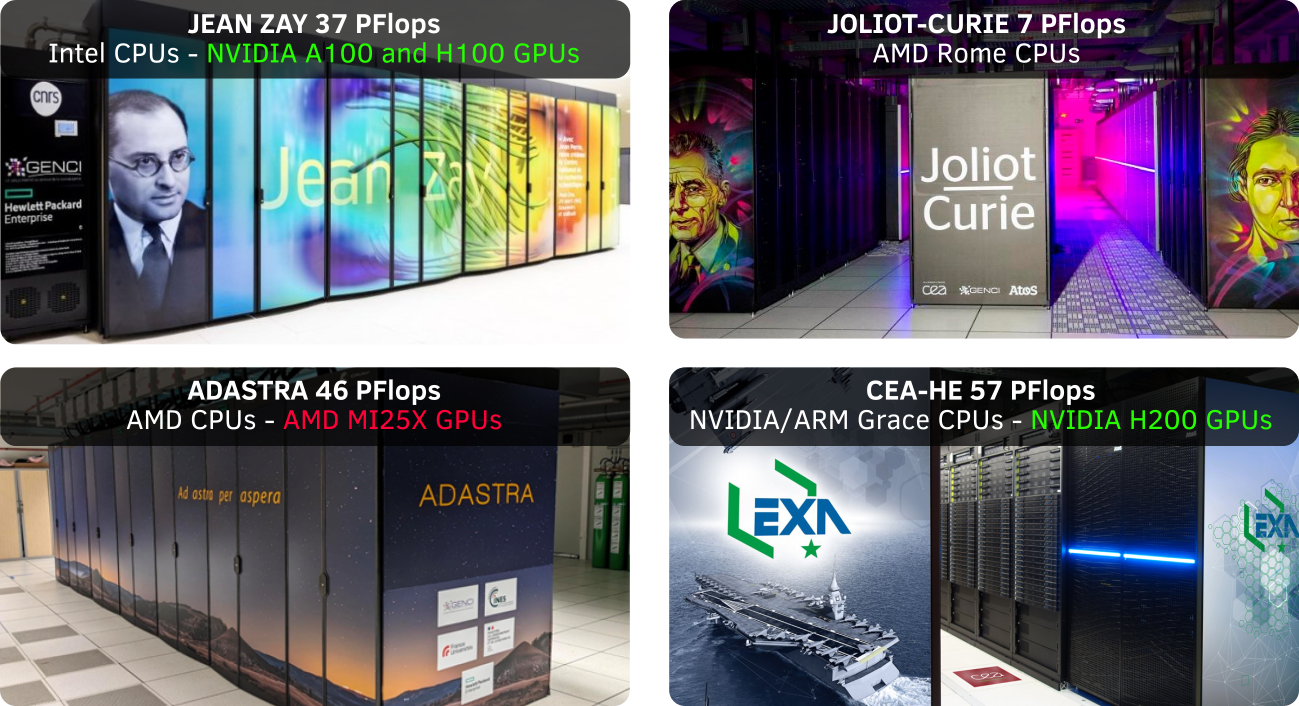
\includegraphics[width=0.9\textwidth]{../../images/french_super_computers.png}
    \caption{Academic and CEA supercomputers}
    \end{center}
\end{figure}

\end{frame}

% _____________________________________________________________________________

\begin{frame}
    \frametitle{Top500 GPU-CPU system share}

\begin{center}
    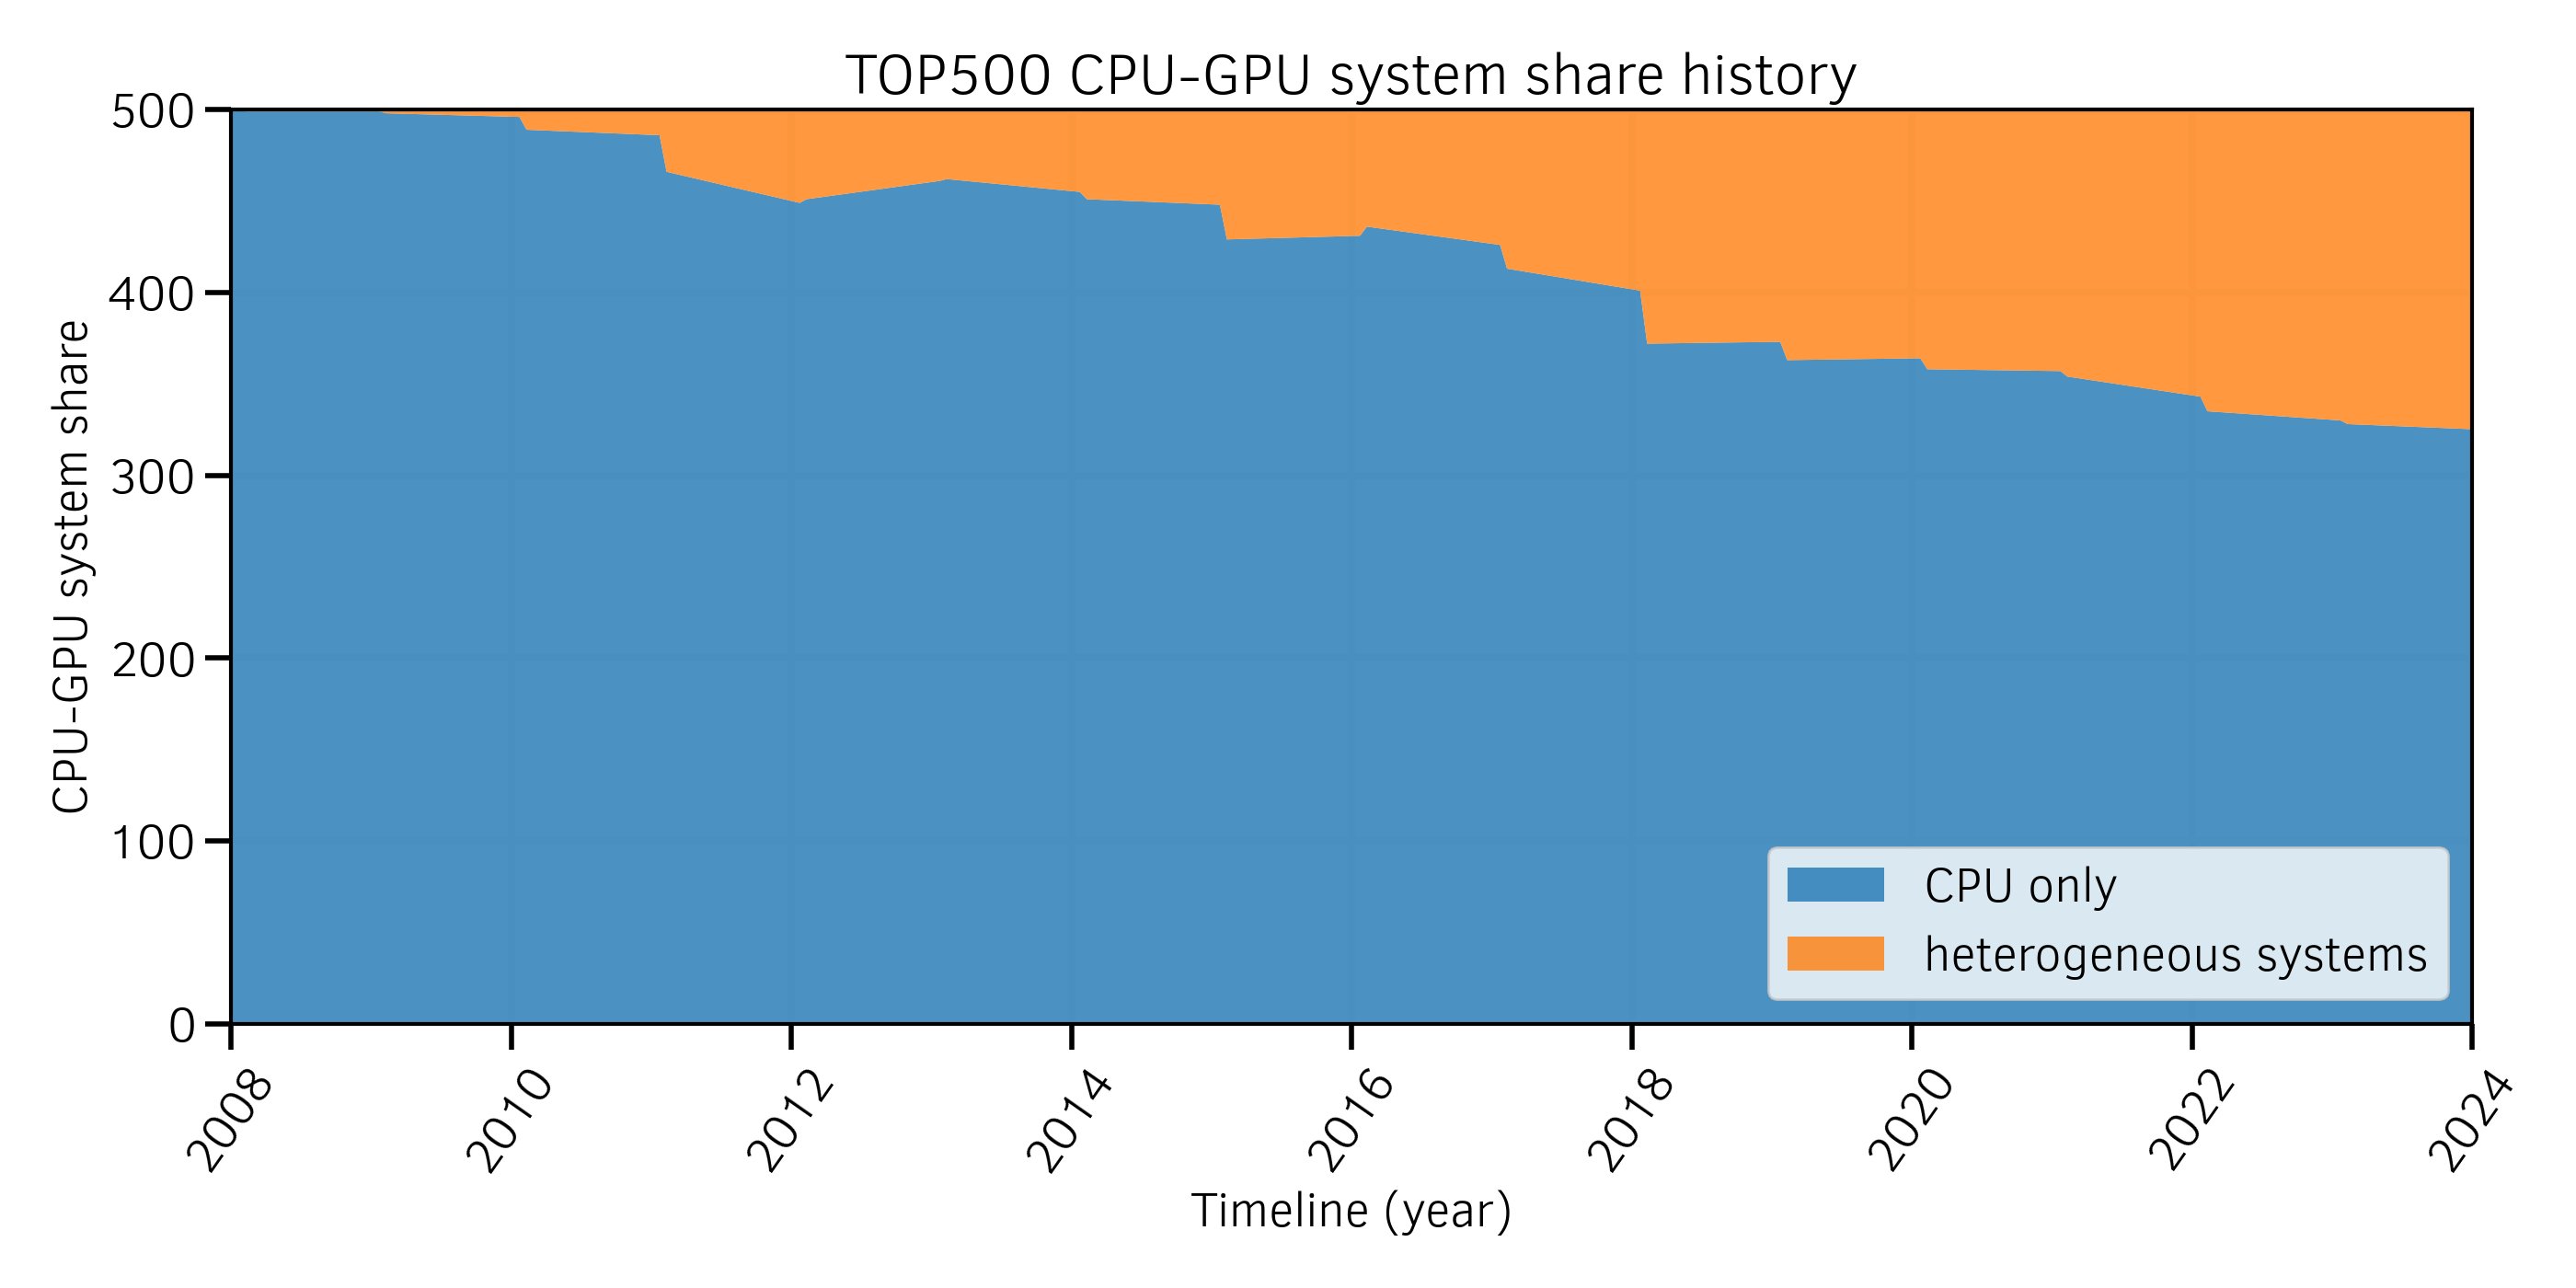
\includegraphics[width=0.9\textwidth]{../../images/top500_cpu_gpu_share_history.png}
\end{center}

\footnotesize
* Does not include exotic and Intel Knight Landing accelerators

\end{frame}

% _____________________________________________________________________________

\begin{frame}
    \frametitle{Basic definition of a supercomputer}

    \begin{itemize}
        \item A supercomputer is a distributed memory system composed of many compute nodes packed into racks and linked by a high-speed network
        \item Compute nodes are composed of one or more CPUs and one or more accelerators
        \item Most common accelerators today are GPGPU for General Purpose Graphic Processing Units
    \end{itemize}

    \begin{center}
        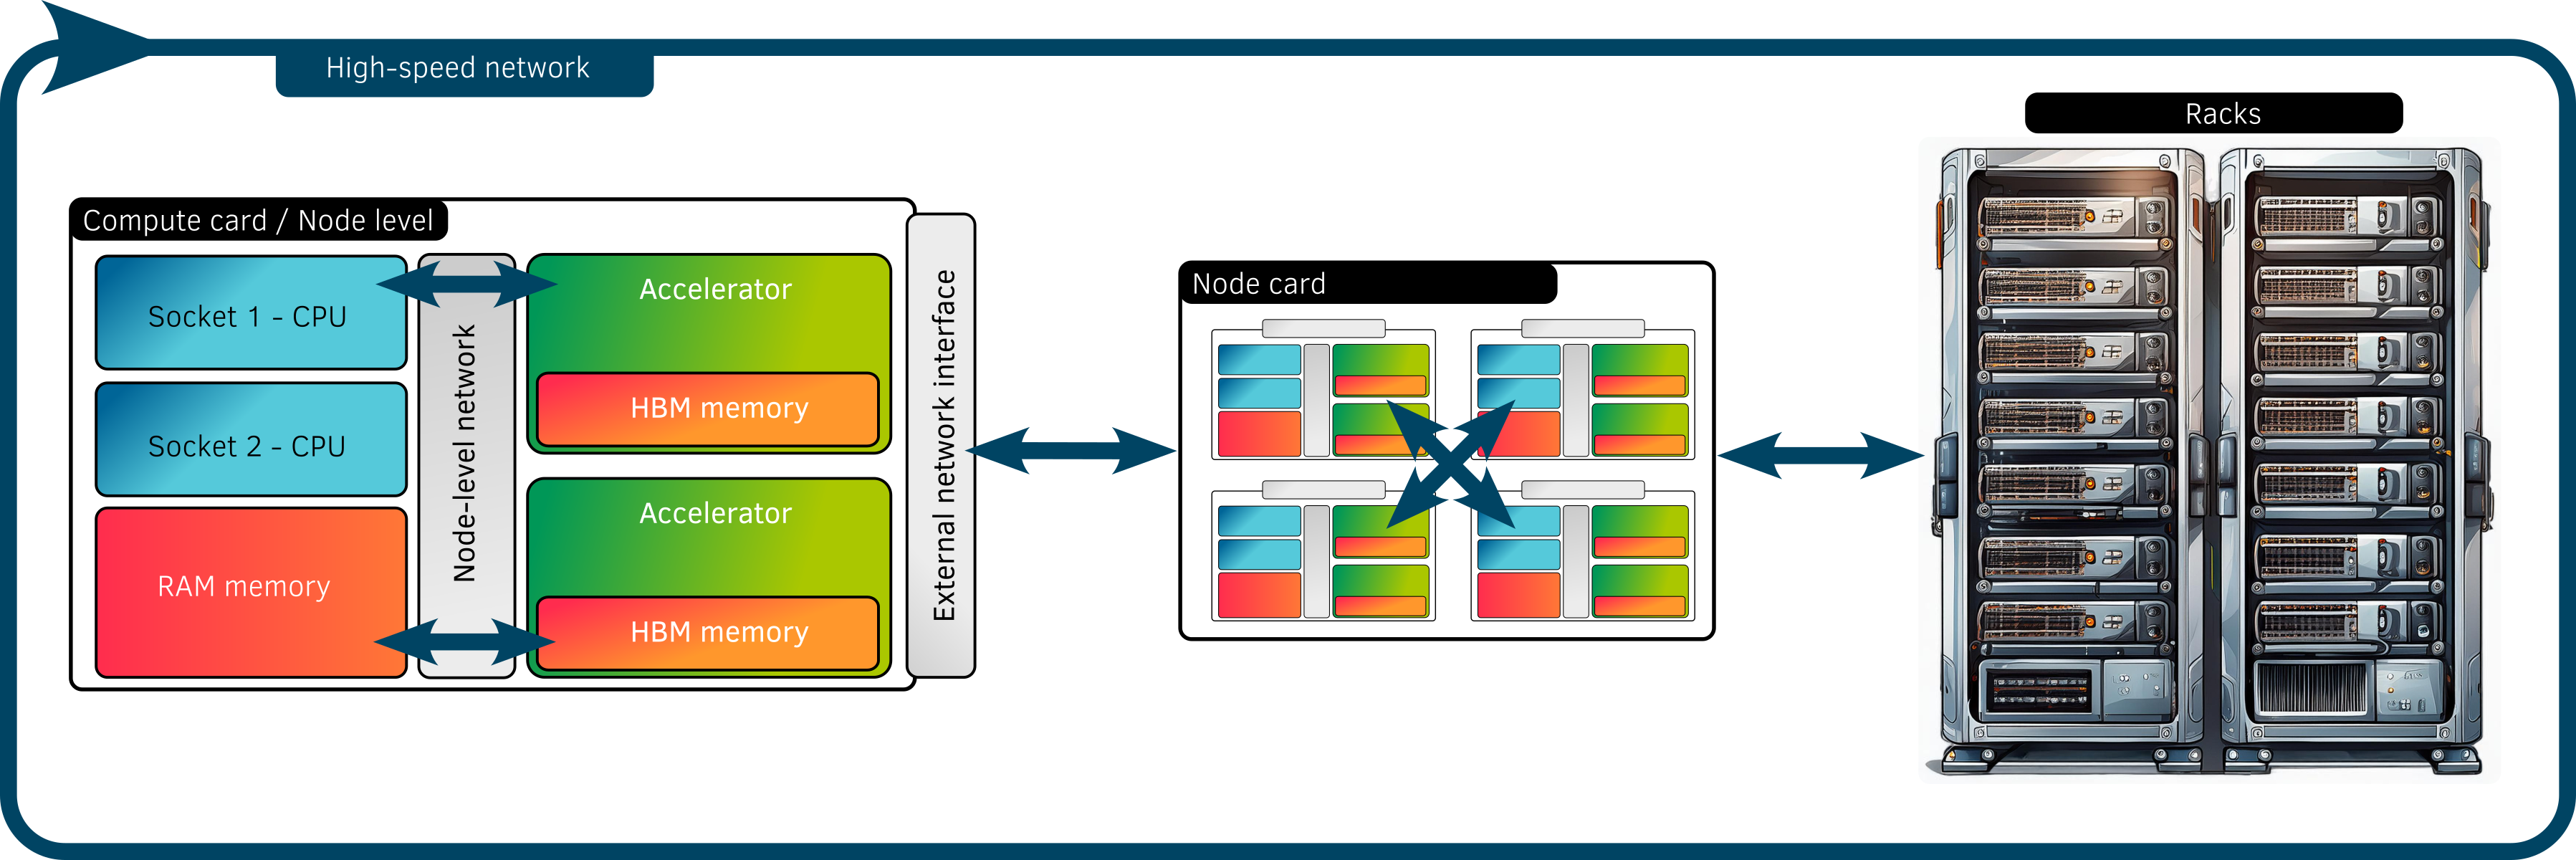
\includegraphics[width=\textwidth]{../../images/super-computer_architecture.png}
    \end{center}

\end{frame}

% _____________________________________________________________________________

\begin{frame}
    \frametitle{Zoom on the CPU architecture}

    \small
    \begin{itemize}
        \item CPUs are designed for general purpose, from sequential task to parallel computing. They run the operating system as well.
        \item Tens to hundred of cores in biggest processors
        \item SIMD (Single Instruction Multiple Data) units for accelerating arithmetic operations
    \end{itemize}
    
    \begin{center}
        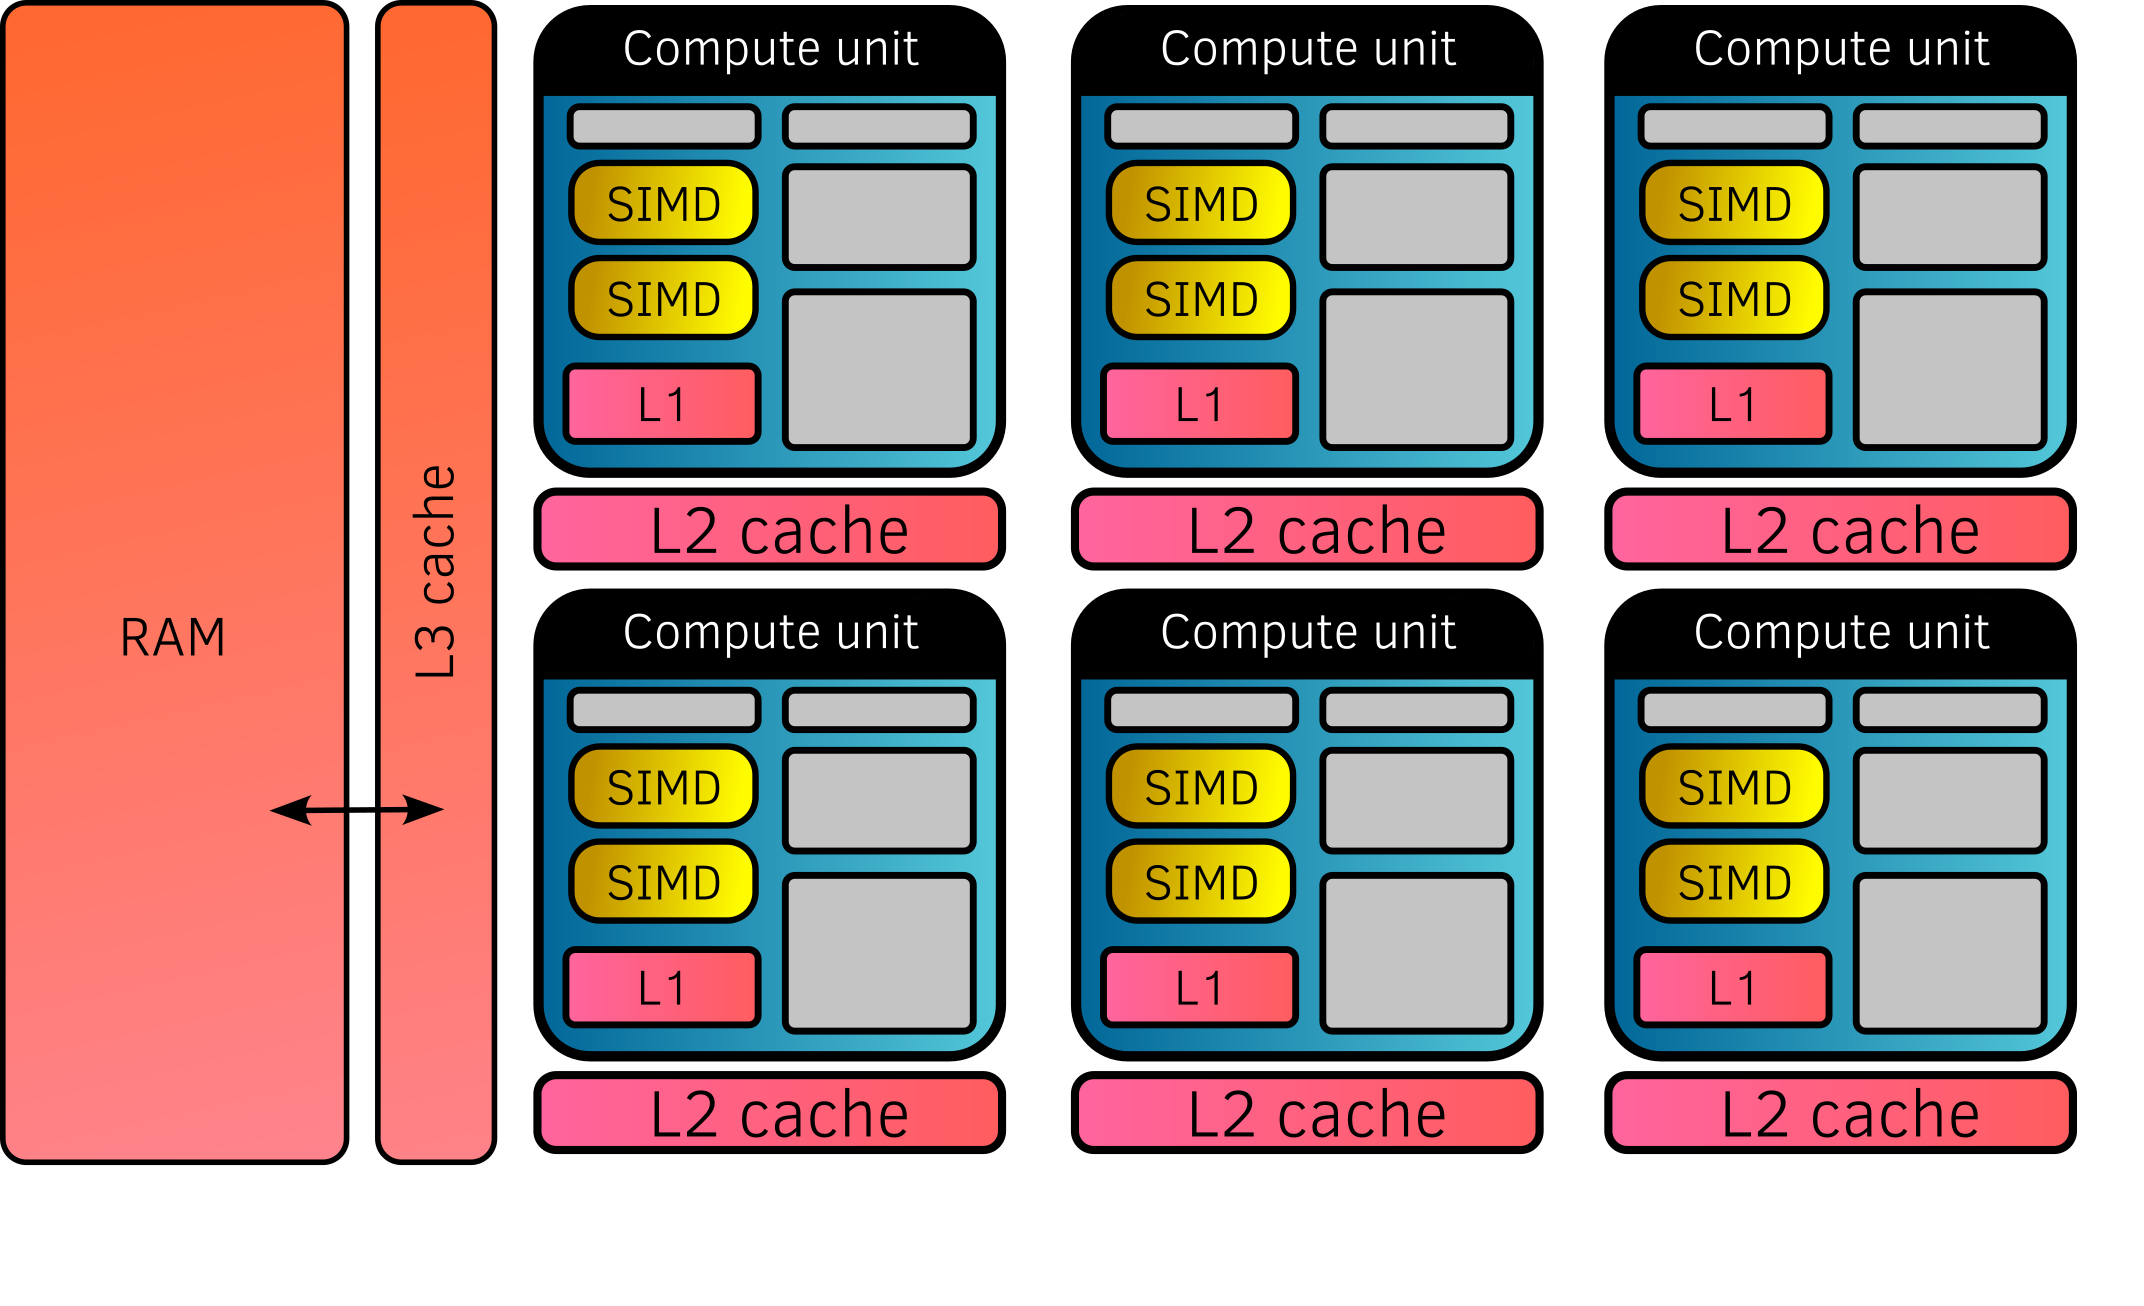
\includegraphics[width=0.7\textwidth]{../../images/cpu_architecture.png}
    \end{center}
    
\end{frame}


% _____________________________________________________________________________

\begin{frame}
    \frametitle{Zoom on the GPGPU architecture}

\small
\begin{itemize}
    \item GPUs are designed to achieve massive parallelism of simple kernels
    \item Hundreds of computing units, thousands of threads
    \item Large SIMT vector unit (Single Instruction Multiple Threads) per computing unit
\end{itemize}

\begin{center}
    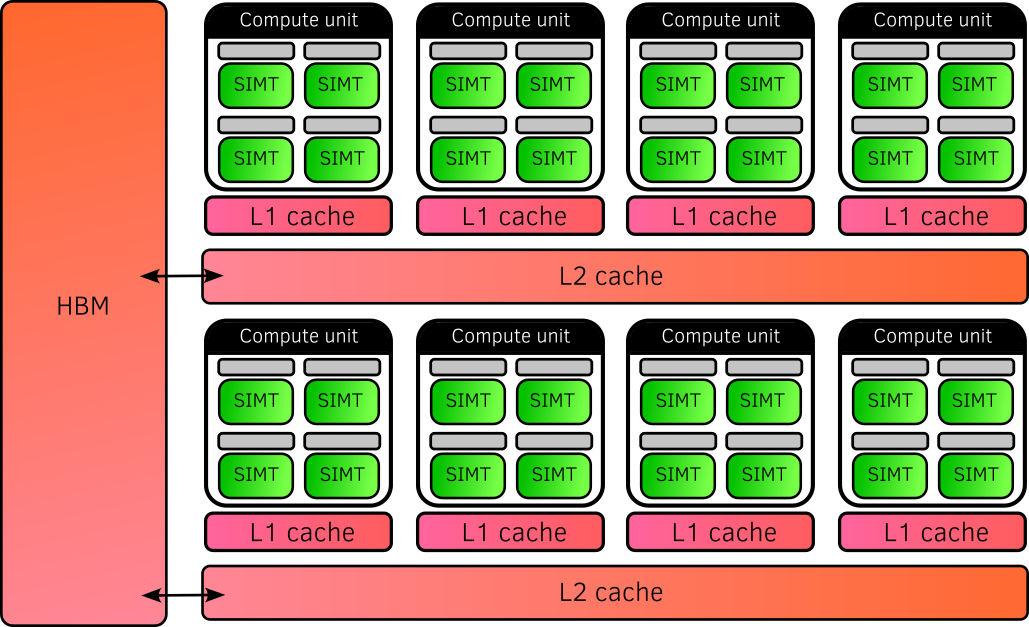
\includegraphics[width=0.7\textwidth]{../../images/gpu_architecture.png}
\end{center}

\end{frame}

% _____________________________________________________________________________

\begin{frame}
    \frametitle{Main difference between CPU and GPU}

    \begin{center}
        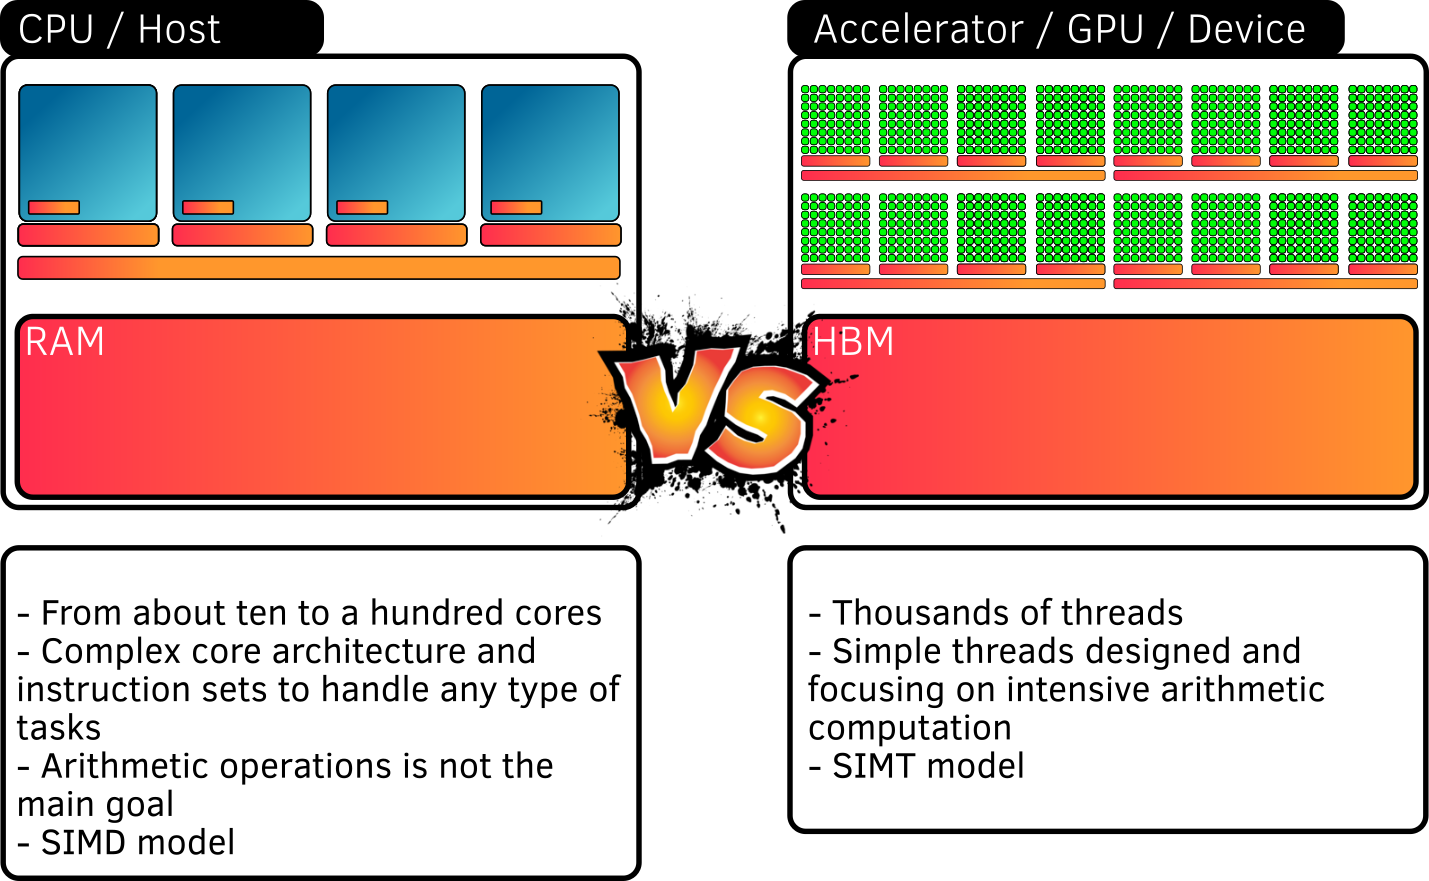
\includegraphics[width=0.8\textwidth]{../../images/cpu_vs_gpu.png}
    \end{center}

\end{frame}

% _____________________________________________________________________________

\begin{frame}
    \frametitle{Host / Device model}

    \begin{itemize}
        \item The program is always started first on the CPU.
        \item The CPU is often referred to as the \highlight{Host}
        \item The CPU orchestrates when the kernels are launched on the GPU and how to make the memory transfers
        \item The GPU side waits for kernels to execute
        \item The GPU is often referred to as the \highlight{Device}
    \end{itemize}

    \begin{alertblock}{}
        Today's GPU can not work standalone
    \end{alertblock}

\end{frame}

% _____________________________________________________________________________

\begin{frame}
    \frametitle{SIMD versus SIMT}

    \begin{center}
        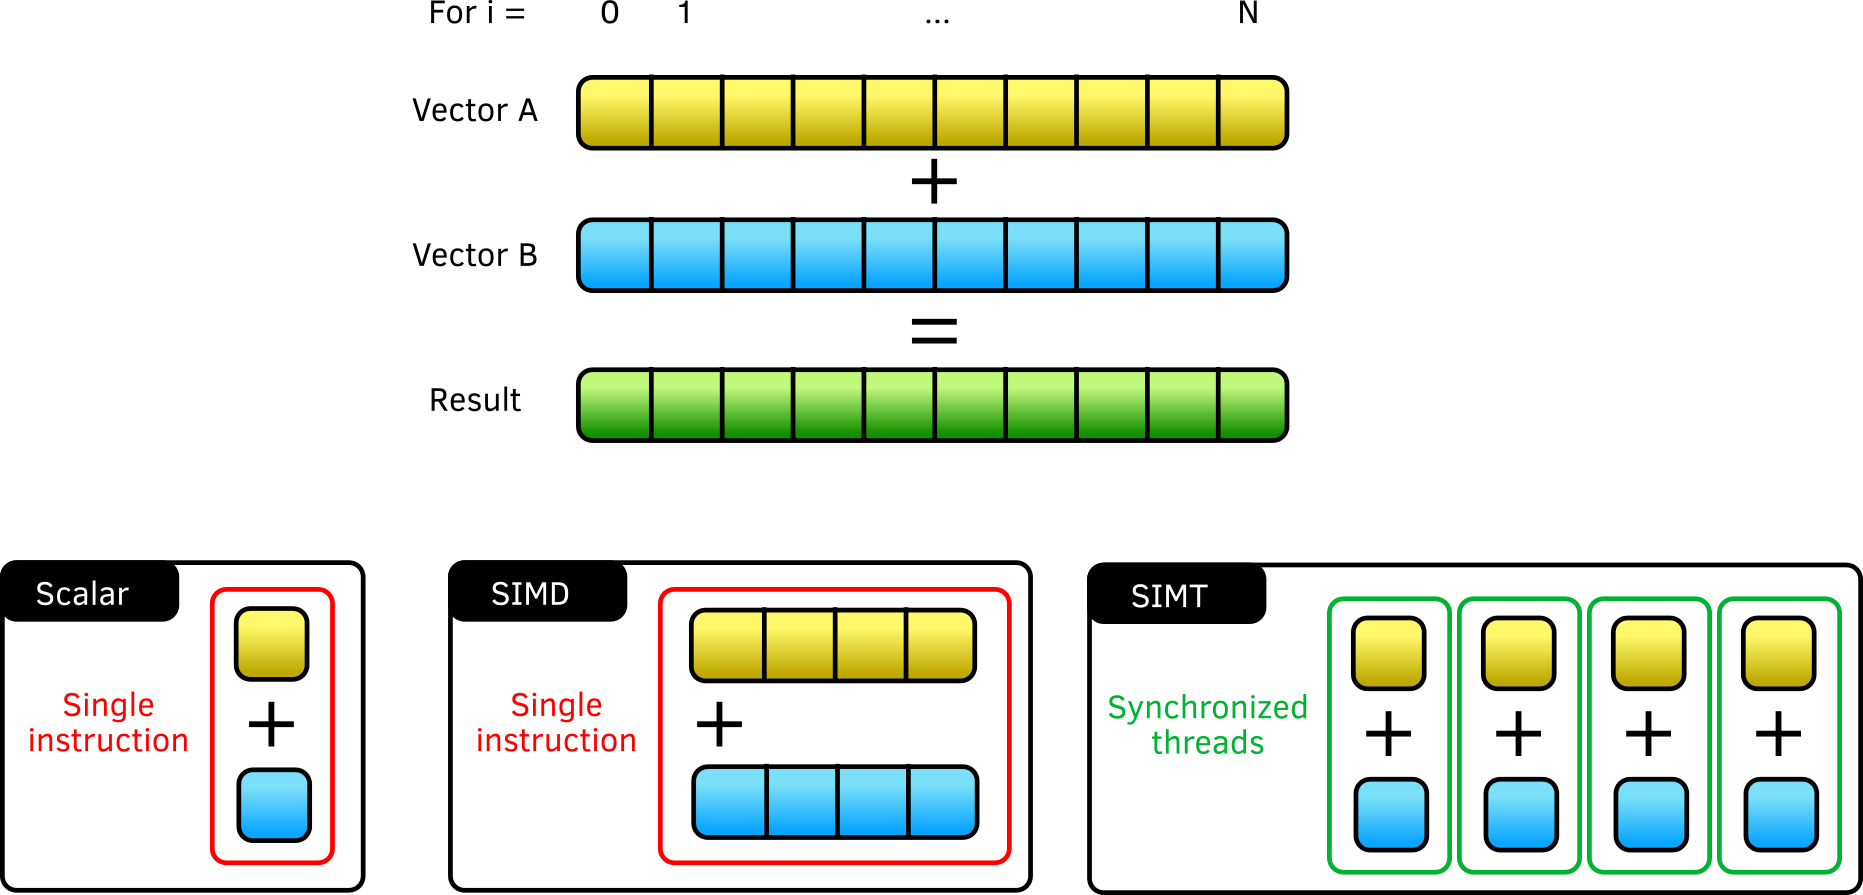
\includegraphics[width=\textwidth]{../../images/SIMD_vs_SIMT.png}
    \end{center}

\end{frame}

% _____________________________________________________________________________

\begin{frame}
    \frametitle{What's the motivation of putting GPUs in supercomputers?}

\begin{center}
    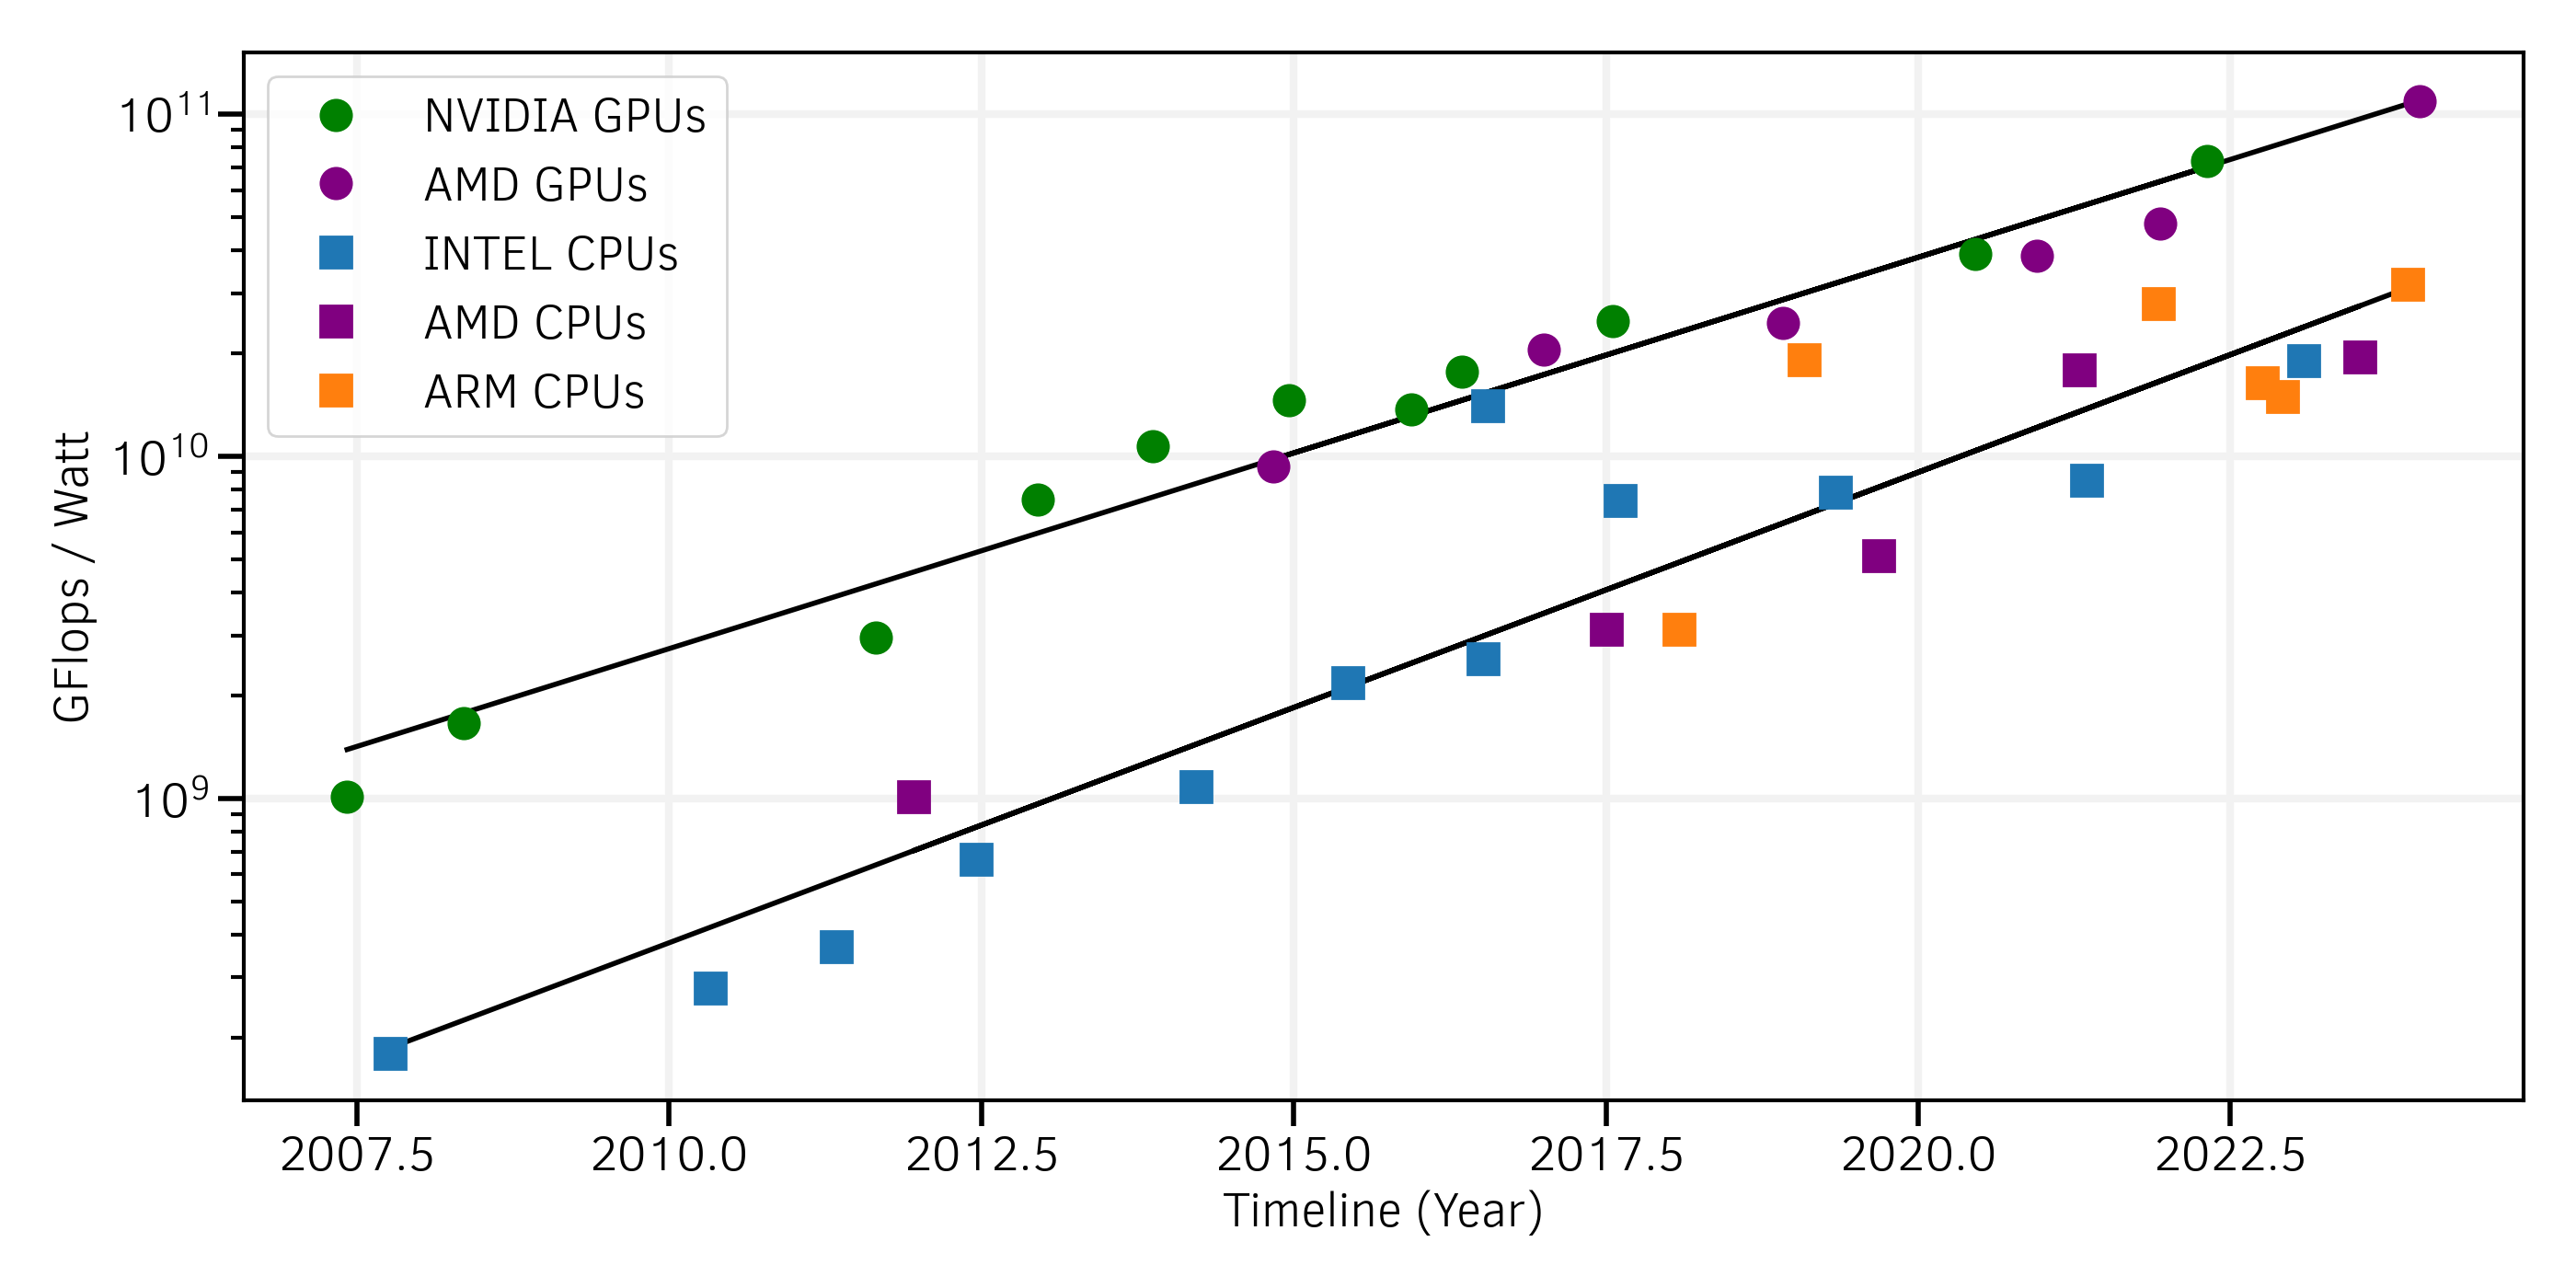
\includegraphics[width=0.9\textwidth]{../../images/flop_watt_ratio_history_fp64.png}
\end{center}

\begin{itemize}
    \item Question: how to build the fastest machine with the lowest power consumption and the lowest cost?
\end{itemize}

\end{frame}

% _____________________________________________________________________________

\begin{frame}
    \frametitle{Parallel programming models and libraries in numerical science}

    \begin{center}
        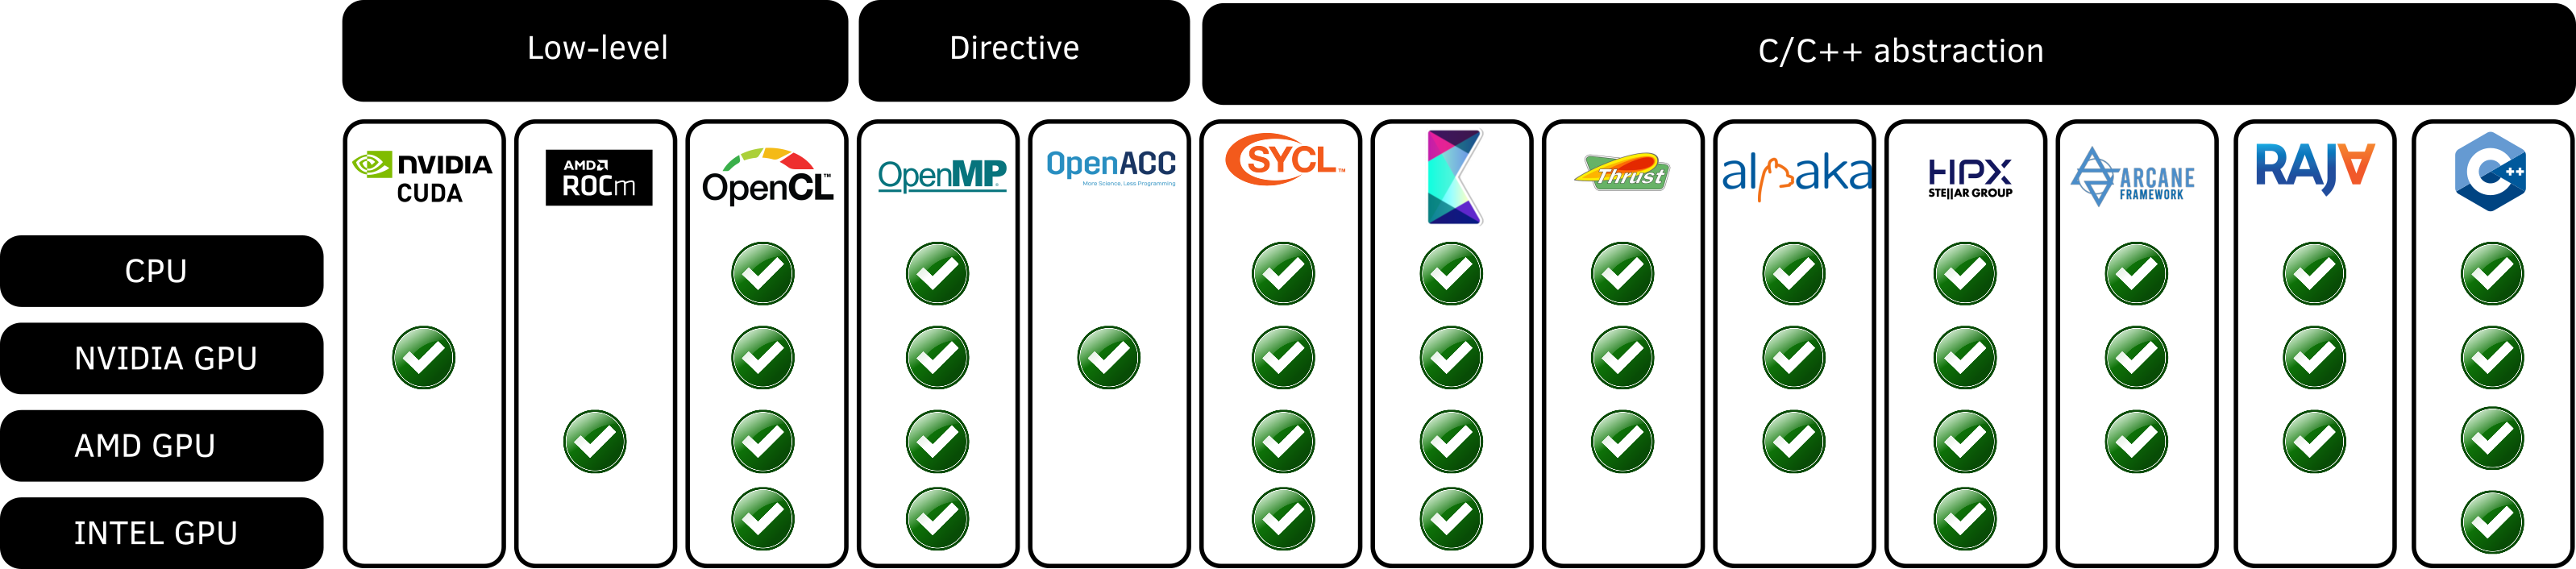
\includegraphics[width=\textwidth]{../../images/prog_model.png}
    \end{center}

    \begin{itemize}
        \item Performance portability is one thing
        \item But we will see that developers need more
    \end{itemize}

\end{frame}

% _____________________________________________________________________________

\begin{frame}
    \frametitle{Performance, Portability and Productivity}

Application developers need:

\begin{itemize}
    \item \textbf{Performance:} the ability to get the best performance on a specific hardware
    \item \textbf{Portability:} the ability to run the same code on different hardware
    \item \textbf{Productivity:} the ability to write code quickly and easily, ability to maintain and extend the code, ability to leverage architecture optimization
\end{itemize}

In the field of numerical simulation, engineers also want:

\begin{itemize}
    \item \textbf{Maturity:} production-ready not research product
    \item \textbf{Community:} contributors, support, documentation, examples
    \item \textbf{Longevity:} long-term maintenance, bug fixes, updates, sponsorship
    \item \textbf{Interporability:} possibility to easily couple with other libraries and tools (IO, Linear Algebra, Machine leaning, etc.)
\end{itemize}

\end{frame}
% _____________________________________________________________________________

\begin{frame}
\frametitle{Do you need performance portability?}
Probably yes if you:
\begin{itemize}
    \item Want your code to run on different hardware technologies (from CPU to GPU)
    \item Have performance requirements
    \item Can not afford to maintain and optimize different versions of your code for each possible hardware of the market
    \item You want to focus on algorithmic and not code development
    \item Want you code to be easily maintainable and readable by others, especially non experts
\end{itemize}

Maybe not if:
\begin{itemize}
    \item Need to tune your algorithms to work as fast as possible on a given hardware
\end{itemize}

\end{frame}

% _____________________________________________________________________________

\begin{frame}
    \frametitle{Kokkos programming model}

    Kokkos is a performance portability parallel programming model build upon the C++-17 standard designed to abstract already-existing parallel programming models.

    \hspace{0.5cm}

    \begin{itemize}
        \item Kokkos provides data structures and functions based on modern C++ to build your application
        \item Developers never directly use underlying backends (no CUDA kernels for instance)
    \end{itemize}

    \begin{center}
        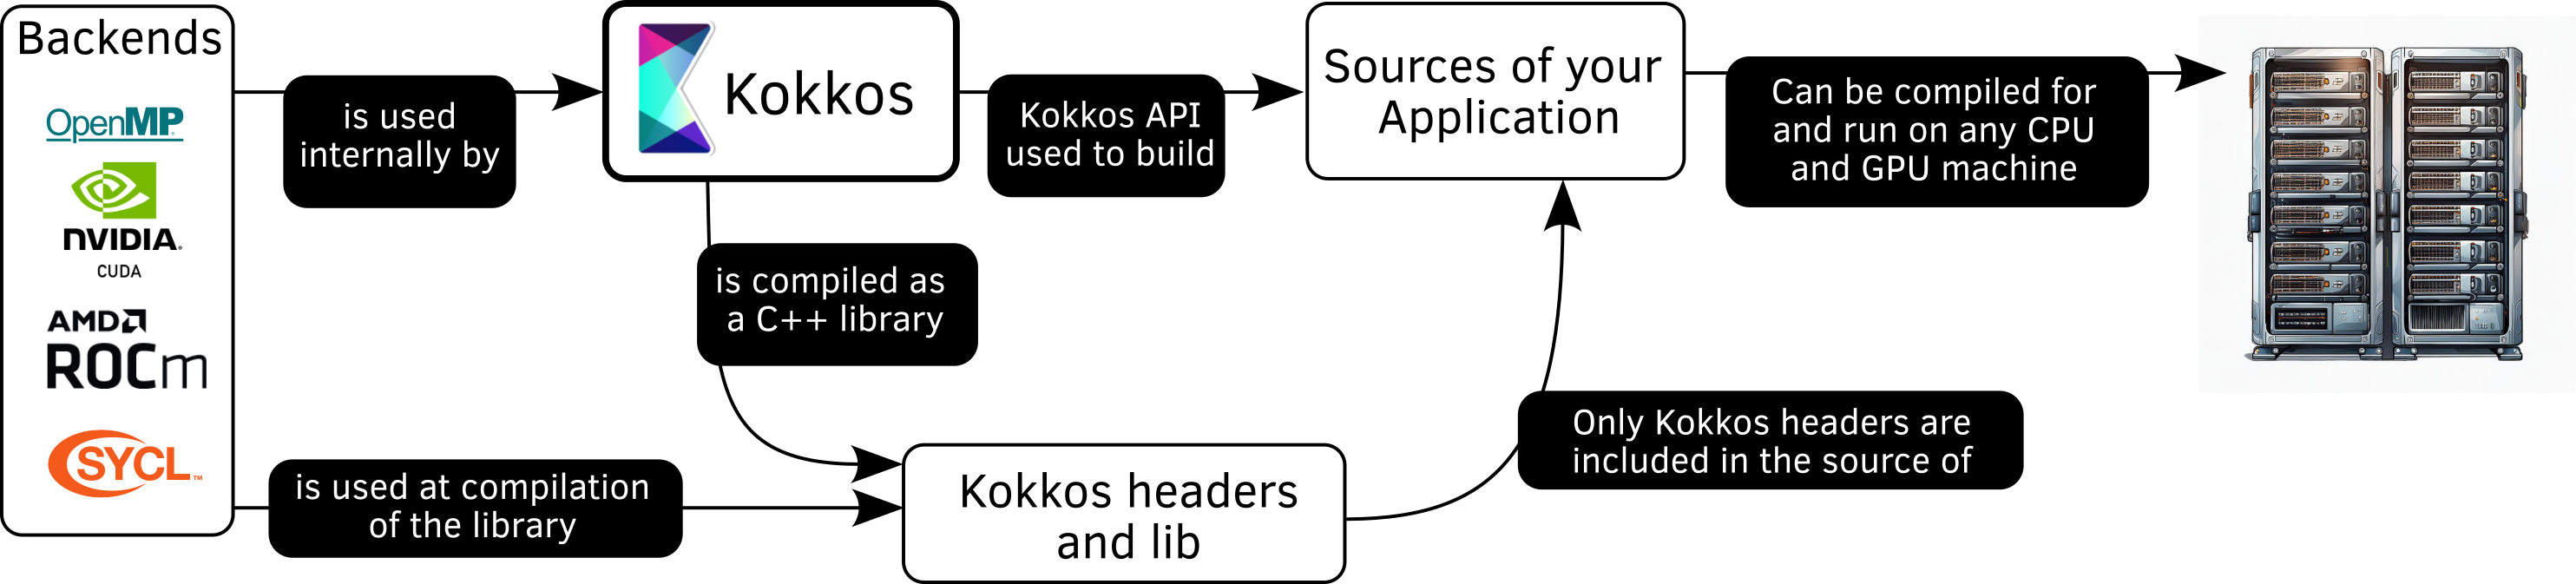
\includegraphics[width=1\textwidth]{../../images/kokkos_model.png}
    \end{center}

\end{frame}

% _____________________________________________________________________________

\begin{frame}
    \frametitle{Kokkos parallelism scope}

    \begin{itemize}
        \item Kokkos only handle node-level parallelism
        \item You still need a model for distributed memory parallelism (MPI for instance)
    \end{itemize}


\end{frame}

% _____________________________________________________________________________

\begin{frame}
    \frametitle{Kokkos: a tool for both C++ beginners and experts} 
    \textbf{Kokkos' basic capabilities:}
    \begin{itemize}
        \item Abstraction of most parallel patterns used in HPC (loops, reduction, scan)
        \item Abstracted basic data structures used in science (vectors, multi-D arrays, sub-arrays, strided arrays, etc)
    \end{itemize}
    \textbf{Kokkos' advanced capabilities:}
    \begin{itemize}
        \item Advanced data structure properties
        \item Thread safety, thread scalability, and atomic operations
        \item Hierarchical patterns for maximizing parallelism 
    \end{itemize}
    \textbf{Kokkos' tools and Kernels:}
    \begin{itemize}
        \item Profiling, tuning and debuging tools
        \item Interacting with Python and Fortran
        \item Library extensions: Kokkos Kernels for Linear Algebra, Kokkos FFT, Kokkos Comm and more 
    \end{itemize}
\end{frame}

% _____________________________________________________________________________

\begin{frame}
    \frametitle{Kokkos ecosystem}

    \begin{center}
        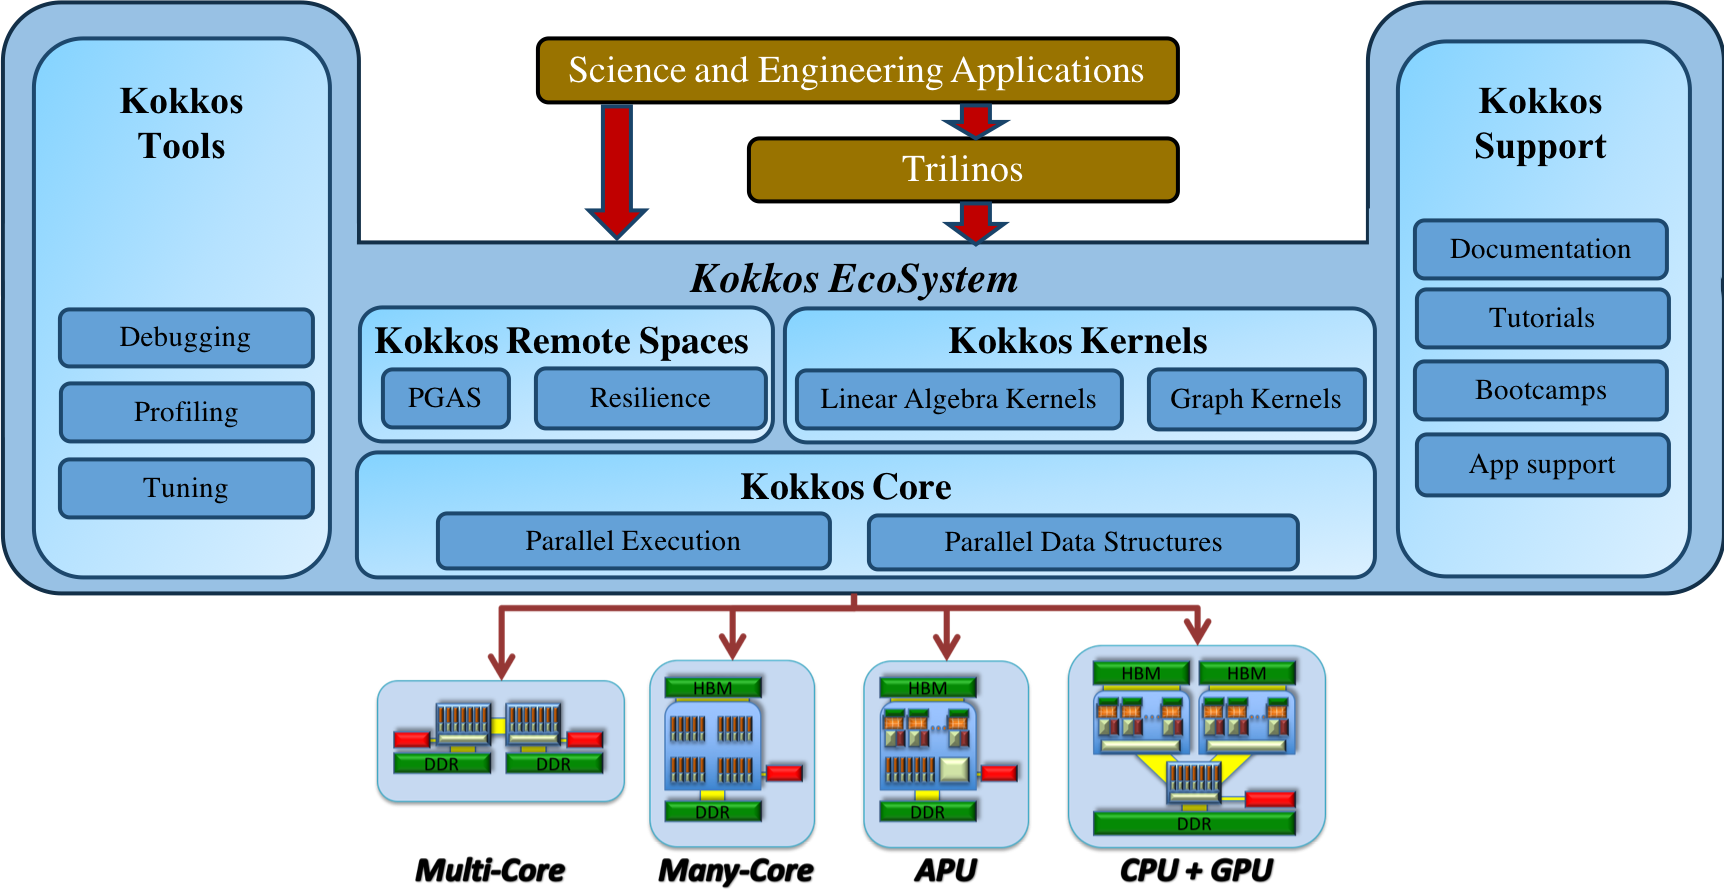
\includegraphics[width=\textwidth]{../../images/kokkos-ecosystem.png}
    \end{center}

\end{frame}

% _____________________________________________________________________________

\begin{frame}
    \frametitle{Kokkos and the evolution of the C++ standard} 
    \begin{center}
        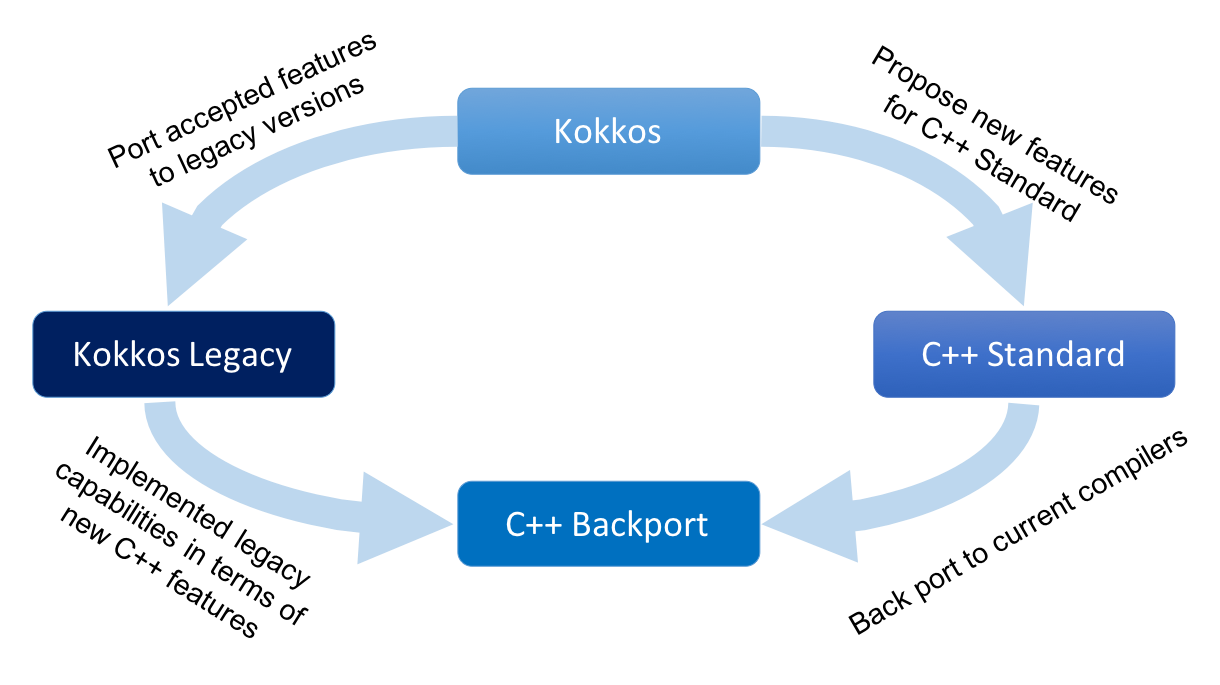
\includegraphics[width=\textwidth]{../../images/kokkos-cpp-standard.png}
    \end{center}
\end{frame}

% _____________________________________________________________________________

\begin{frame}
    \frametitle{Kokkos useful resources} 
    \begin{itemize}
        \item Kokkos GitHub: \href{https://github.com/kokkos}{https://github.com/kokkos}
        \item Documentation: \href{https://kokkos.org/kokkos-core-wiki/}{https://kokkos.org/kokkos-core-wiki/}
        \item Cheat sheet: \href{https://github.com/CExA-project/cheat-sheet-for-kokkos/blob/main/README.md}{https://github.com/CExA-project/cheat-sheet-for-kokkos/blob/main/README.md}
        \item Slack channel: \href{https://kokkosteam.slack.com/}{https://kokkosteam.slack.com/}
    \end{itemize}
\end{frame}

% _____________________________________________________________________________

\section{Basic concepts of Kokkos}

\begin{frame}
    \centering
    \Huge Basic concepts of Kokkos
\end{frame}

% _____________________________________________________________________________

\subsection[Compilation]{Compilation}

% _____________________________________________________________________________

\begin{frame}
    \frametitle{Compiling Kokkos from source} 
    \begin{itemize}
        \item Require CMake and a C++ compiler
        \item Compile Kokkos as an external library or as part of your project (inline build) using the source
        \item You can use Spack to install Kokkos
        \item You can get the source code from the \href{https://github.com/kokkos/kokkos}{Kokkos GitHub repository}
    \end{itemize}

    \hspace{1cm}

    \centering
    
\includegraphics[width=0.3\textwidth]{../../images/spack.png}
    
\includegraphics[width=0.3\textwidth]{../../images/GitHub-logo.png}

\end{frame}

% _____________________________________________________________________________

\begin{frame}
    \frametitle{The notion of backend in Kokkos} 
    \begin{itemize}
        \item Kokkos is compiled to target a specific backend
        \item Only one CPU backend and one GPU backend maximum can be compiled at a time
        \item Kokkos is portable until you compile it. You need one compilation per backend.
    \end{itemize}

    \hspace{1cm}

    \centering
    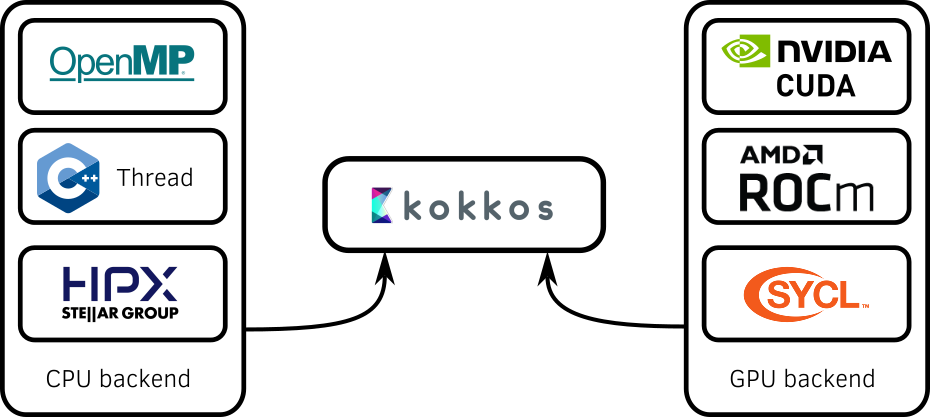
\includegraphics[width=0.75\textwidth]{../../images/kokkos_backend.png}

\end{frame}

% _____________________________________________________________________________

\begin{frame}[fragile]
    \frametitle{Compiling Kokkos with the default parameters} 

\begin{itemize}
    \item Install Kokkos with the serial backend
    \item Use the default compiler or specify with \texttt{-DCMAKE\_CXX\_COMPILER}
\end{itemize}

\begin{minted}[texcomments]{bash}
cmake ${srcdir} \
-DCMAKE_CXX_COMPILER=g++ \
-DCMAKE_INSTALL_PREFIX=${kokkos_install_folder}
\end{minted}

\end{frame}

% _____________________________________________________________________________

\begin{frame}[fragile]
    \frametitle{Compiling Kokkos for a specific backend} 

\begin{itemize}
    \item Add the cmake option \texttt{-DKokkos\_ENABLE\_<BACKEND>=ON} to enable a specific backend, replacing \texttt{<BACKEND>} with the backend name
\end{itemize}
\small
\begin{minted}[texcomments]{bash}
cmake ${srcdir} \
-DCMAKE_CXX_COMPILER=g++ \ 
-DCMAKE_INSTALL_PREFIX=${kokkos_install_folder} \
-DKokkos\_ENABLE\_<BACKEND>=ON
\end{minted}
\normalsize
\begin{itemize}
    \item Serial backend is \texttt{SERIAL}
    \item CPU backends are \texttt{OPENMP}, \texttt{THREADS}, \texttt{HPX}
    \item GPU backends are \texttt{CUDA}, \texttt{HIP}, \texttt{SYCL}, \texttt{OPENMPTARGET}
\end{itemize}   

\end{frame}

% _____________________________________________________________________________

\begin{frame}[fragile]
    \frametitle{Warning regarding the Kokkos compilation}

    \begin{alertblock}{}
        All backends do not have the same level of maturity, some are experimental
    \end{alertblock}

    \begin{alertblock}{}
        Backend (for instance CUDA) must be available on the target machine and in the environment, Kokkos does not install it for you
    \end{alertblock}

\end{frame}

% _____________________________________________________________________________

\begin{frame}[fragile]
    \frametitle{Compiling Kokkos for a specific archiecture}

\begin{itemize}
    \item Architecture cmake options \texttt{-DKokkos\_ARCH\_<ARCH\_NAME>=ON} can be specified for best performance
    \item Replace \texttt{<ARCH\_NAME>} with the architecture name of the target host and device
    \item For example, for a NVIDIA A100 GPU, the architecture name is \texttt{AMPERE80}
    \item All Cmake options are available \href{https://kokkos.org/kokkos-core-wiki/keywords.html#}{on the dedicated doc page}
\end{itemize}

\end{frame}

% _____________________________________________________________________________

\begin{frame}[fragile]
    \frametitle{Example: compiling Kokkos for a node with a multi-core Xeon Skylake CPU and a A100 NVIDIA GPU} 

\begin{itemize}
    \item We use OpenMP for the multi-core CPU and CUDA for the NVIDIA GPU
    \item We add the A100 Kokkos option for the best performance \texttt{-DKokkos\_ARCH\_AMPERE80=ON}
    \item We add the Skylake option, mostly for vectorization \texttt{-DKokkos\_ARCH\_SKX=ON}
\end{itemize}

\footnotesize
\begin{minted}[texcomments]{bash}
cmake ${srcdir} -DCMAKE_INSTALL_PREFIX=${kokkos_install_folder} \
-DKokkos_ENABLE_OPENMP=ON -DKokkos_ENABLE_CUDA=ON \
-DKokkos_ARCH_AMPERE80=ON -DKokkos_ARCH_SKX=ON
\end{minted}

\hspace{0.5cm}

\centering
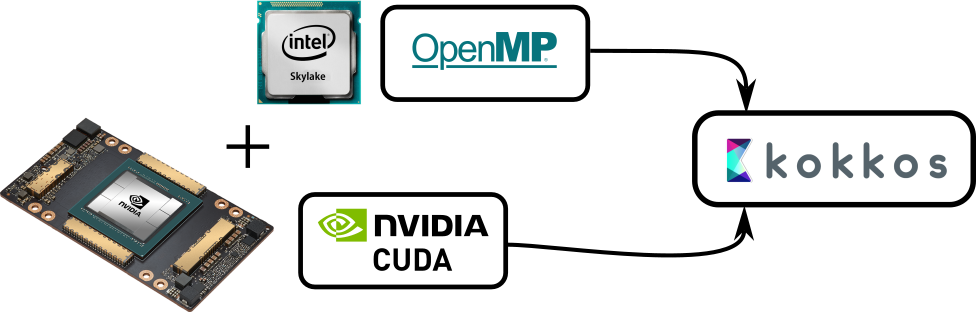
\includegraphics[width=0.7\textwidth]{../../images/kokkos_a100_backend.png}

\end{frame}
% _____________________________________________________________________________

\begin{frame}[fragile]
    \frametitle{Exercise 1: learn how to compile Kokkos}

    \begin{center}
    
\includegraphics[width=0.4\textwidth]{../../images/sleeping_otter.png}
    \end{center}

    Go to the folder \href{https://github.com/CExA-project/cexa-kokkos-tutorials/tree/main/exercises/01_compiling_kokkos}{01\_compiling\_kokkos} and follow the instructions in the README file

    Goal of this Exercise:
    \begin{itemize}
        \item Compile Kokkos with the default parameters
        \item Compile Kokkos with the OpenMP backend
        \item Compile Kokkos with a GPU backend
    \end{itemize}

\end{frame}

% _____________________________________________________________________________

\subsection[Starting a Kokkos program]{Starting and compiling a Kokkos program}

% _____________________________________________________________________________

\begin{frame}[fragile]
    \frametitle{Start a Kokkos program}
    \begin{itemize}
        \item Include the Kokkos header file (like any other library)
        \item Use the Kokkos namespace \texttt{Kokkos::}
        \item Initialize and finalize Kokkos (like MPI)
    \end{itemize}

\begin{minted}{C++}
#include <Kokkos_Core.hpp>

int main(int argc, char* argv[]) {
    Kokkos::initialize(argc, argv);
    {
        // Your code here
    }
    Kokkos::finalize();
    return 0;
}
\end{minted}

\end{frame}

% _____________________________________________________________________________

\begin{frame}[fragile]
    \frametitle{ScopeGuard: an alternative to initialize and finalize} 

    \begin{itemize}
        \item ScopeGuard is a class that ensure thats Kokkos::initialize and Kokkos::finalize are called correctly.
        \item It is a Resource Acquisition Is Initialization pattern
    \end{itemize}

\begin{minted}{C++}
#include <Kokkos_Core.hpp>
    
int main(int argc, char* argv[]) {
    Kokkos::ScopeGuard guard(argc, argv);
        
    // Your code here
}
\end{minted}

\end{frame}

% _____________________________________________________________________________

\begin{frame}[fragile]

\frametitle{Use CMake to compile your Kokkos program}

\begin{itemize}
    \item Kokkos should be compiled and installed on your system
    \item Use the \texttt{find\_package} CMake command to find Kokkos
    \item Use the \texttt{target\_link\_libraries} CMake command to link your program with Kokkos
\end{itemize}

\begin{minted}[texcomments]{cmake}
cmake_minimum_required (VERSION 3.12)
project(my_kokkos_project LANGUAGES CXX)
find_package(Kokkos REQUIRED)
add_executable(test main.cpp)
target_link_libraries(test Kokkos::kokkos)
\end{minted}

\end{frame}

% _____________________________________________________________________________

\begin{frame}[fragile]

\frametitle{Use CMake to compile your Kokkos program}

\begin{itemize}
    \item Kokkos propagates its compilation flags to your program
    \item If Kokkos is not detected in your paths, use the \texttt{Kokkos\_ROOT} CMake variable to specify the path to Kokkos
\end{itemize}

\small
\begin{minted}[texcomments]{bash}
cmake ${srcdir} \
  -DKokkos_ROOT=${kokkos_install_prefix} \
  -DCMAKE_CXX_COMPILER=${compiler_used_to_build_kokkos}
\end{minted}

\end{frame}

% _____________________________________________________________________________

\begin{frame}[fragile]
    \frametitle{Exercise 2: learn how to compile a Kokkos program} 

    \begin{center}
    
\includegraphics[width=0.4\textwidth]{../../images/sleeping_otter.png}
    \end{center}

    Go to the folder \href{https://github.com/CExA-project/cexa-kokkos-tutorials/tree/main/exercises/02_first_program}{02\_first\_program} and follow the instructions in the README file

    Goal of this Exercise:

    \begin{itemize}
        \item Write a simple Kokkos program
        \item Compile the program with CMake
    \end{itemize}

\end{frame}


% _____________________________________________________________________________

\subsection[Data container]{View: an abstracted data container}

% _____________________________________________________________________________

\begin{frame}[fragile]
    \frametitle{Kokkos has an abstracted data container called View} 

Why is it important to have an abstracted data container?

\begin{itemize}
    \item No need to allocate or deallocate memory by hand
    \item Vendor-specific memory allocation is hidden
    \item Unified semantic and portable memory management (CPU and GPU)
    \item Advanced capability (abstracted layout, subarray, multidimensionality, etc.)
\end{itemize}

Kokkos provides the notion of view:

\begin{itemize}
    \item View is an abstraction of the notion of vector (resize function for instance) and multi-dimensional array
    \item Bring portable Python numpy-like syntax (and Fortran multi-dimensional array)
\end{itemize}

\end{frame}

% _____________________________________________________________________________

\begin{frame}[fragile]
    \frametitle{Creating a dynamic View}

\begin{itemize}
    \item View is a template class
    \item Number of dimensions fixed at compilation time
    \item Size of each dimension determined at runtime
\end{itemize}

\footnotesize
\begin{minted}[texcomments]{C++}
Kokkos::View<class DataType*> view (const std::string name, 
                                    const int size_0, 
                                    const int size_1, ...);
\end{minted}

Template arguments:

\begin{itemize}
    \item \texttt{DataType}: can be any C++ type (\texttt{int}, \texttt{float}, \texttt{double}, etc)
    \item \texttt{*}: add a star per dimension
\end{itemize}

Runtime arguments:

\begin{itemize}
    \item \texttt{name}: Name of the view
    \item \texttt{size\_0}: Size of the first dimension
    \item \texttt{size\_1}: Size of the second dimension
\end{itemize}


\end{frame}

% _____________________________________________________________________________

\begin{frame}[fragile]
    \frametitle{Examples}

\small
\begin{minted}[texcomments]{C++}
const int Nx = 1000;
const int Ny = 2000;

// Vector of double of size Nx
Kokkos::View<double*> my_view("vector", Nx);

// Matrix of int of size Nx x Ny
Kokkos::View<int**> my_matrix("matrix", Nx, Ny);
\end{minted}

\end{frame} 

% _____________________________________________________________________________

\begin{frame}[fragile]
    \frametitle{Accessing the data}

\begin{itemize}
    \item Data can be accessed using the parenthesis operator \texttt{(i,j,k,...)}
    \item Raw data can be accessed using the \texttt{data()} method (not recommended)
\end{itemize}

Example accessing the data on Host:

\small
\begin{minted}[texcomments]{C++}
const int Nx = 1000;
const int Ny = 2000;
Kokkos::View<int**> my_matrix("matrix", Nx, Ny);
for (int i = 0; i < Nx; i++) {
    for (int j = 0; j < Ny; j++) {
        my_matrix(i,j) = i + j;
    }
}
\end{minted}

\end{frame} 

% _____________________________________________________________________________

\begin{frame}[fragile]
    \frametitle{Where does the data reside?}

    \begin{itemize}
        \item A View lives in a specific memory space (Host or Device) not both
        \item If Kokkos is compiled with \highlight{a CPU backend only}, the View data is allocated in the \highlight{Host memory} by defaults
    \end{itemize}

    \centering
    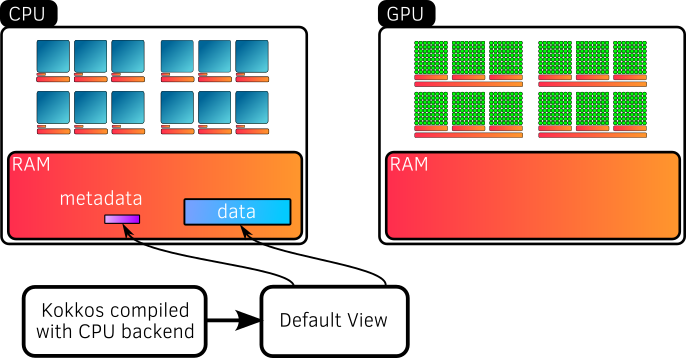
\includegraphics[width=0.7\textwidth]{../../images/host_view_memory.png}

\end{frame} 

% _____________________________________________________________________________

\begin{frame}[fragile]
    \frametitle{Where does the data reside?}

    \begin{itemize}
        \item If Kokkos is compiled with a \highlight{GPU backend}, the View data is allocated in the \highlight{Device memory} by default
        \item We will later see how to allocate and copy data between the Host and the Device
    \end{itemize}

\centering
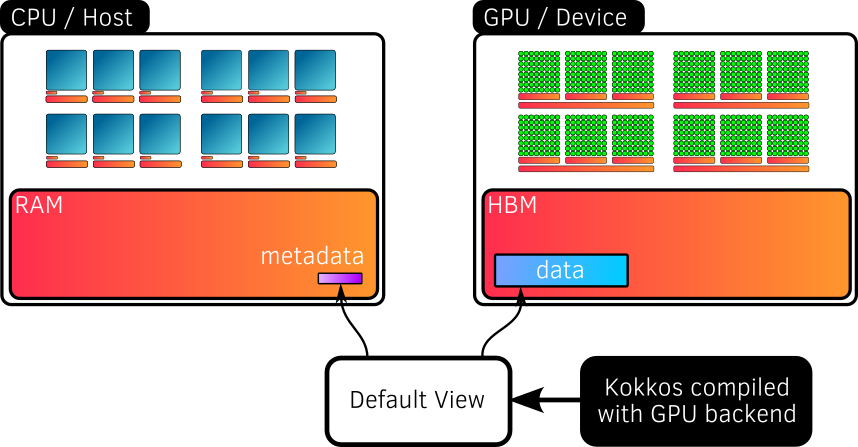
\includegraphics[width=0.7\textwidth]{../../images/device_view_memory.png}

\begin{alertblock}{}
    Device view data can not be accessed on the Host and vice versa
\end{alertblock} 

\end{frame} 

% _____________________________________________________________________________

\begin{frame}[fragile]
    \frametitle{More about dynamic views}

\begin{itemize}
    \item Allocations only happen when explicitly specified
    \item Copy construction and assignment are shallow. So, you pass Views by value, not by reference. (Python like)
    \item Reference counting is used for automatic deallocation (like shared pointers)
    \item Metadata (rank, extent, etc) is however always accessible on the Host
\end{itemize}

\begin{alertblock}{}
    Views have a limited number of dimensions (up to 7)
\end{alertblock}

\end{frame} 

% _____________________________________________________________________________

\begin{frame}[fragile]
    \frametitle{Useful methods to manage View}

\begin{itemize}
    \item \texttt{rank()}: return the rank of the view (number of dimensions)
    \item \texttt{extent(const int dim)}: return the size of a specific dimension
    \item \texttt{size()}: return the total number of elements
    \item many others but not the subject of this introduction
\end{itemize}

\end{frame}

% _____________________________________________________________________________

\begin{frame}[fragile]
    \frametitle{Notion of View layout}

\begin{itemize}
    \item Layout is the way to map multidimensional index to memory
    \item Kokkos provides an abstraction of the data layout
    \item The default layout of a View depends on the backend (Host or Device)
    \item How to manipulate the layout is not the subject of this introduction
\end{itemize}

\begin{center}
    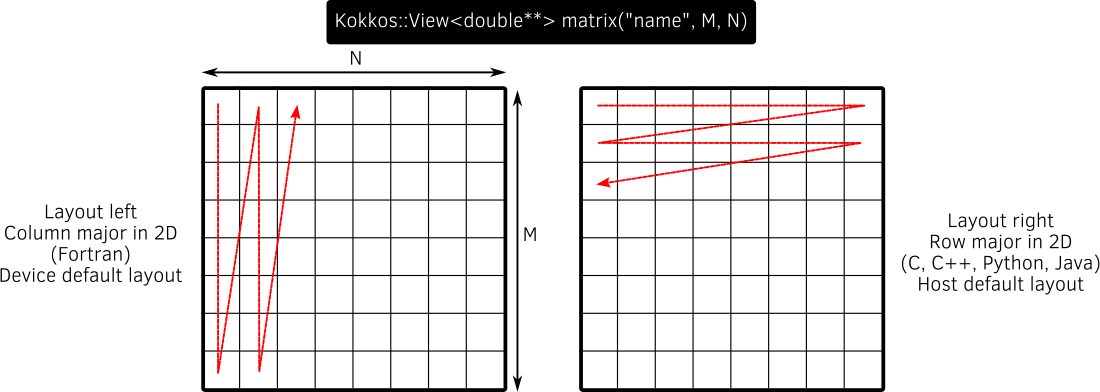
\includegraphics[width=0.95\textwidth]{../../images/layout_right_left.png}
    \end{center}

\end{frame}

% _____________________________________________________________________________


\begin{frame}[fragile]
    \frametitle{Exercise 3: learn how to use a View} 

    \begin{center}
    
\includegraphics[width=0.4\textwidth]{../../images/sleeping_otter.png}
    \end{center}

    Goal of this exercise:

    \begin{itemize}
        \item Create and manage a View
    \end{itemize}

    \begin{block}{}
        Go to the exercise \href{https://github.com/CExA-project/cexa-kokkos-tutorials/tree/main/exercises/03_basic_view}{03\_basic\_view} and follow the instructions in the README file
    \end{block}

\end{frame}

% _____________________________________________________________________________

\begin{frame}[fragile]
    \frametitle{Understand the notion of memory space}

\begin{itemize}
    \item Kokkos provides an abstraction of where the data lives: \textbf{the memory space}
    \item A View is always associated with a defined memory space (Host or Device for instance) at compilation time
    \item Default behavior: View data is allocated in the Host memory space if no GPU backend is available, else in the Device memory space
\end{itemize}
\end{frame}

% _____________________________________________________________________________

\begin{frame}[fragile]
    \frametitle{Understand the notion of memory space}

\begin{itemize}
    \item \textbf{Problem:} how to deal with data residing in different memory spaces?
\end{itemize}

\begin{center}
    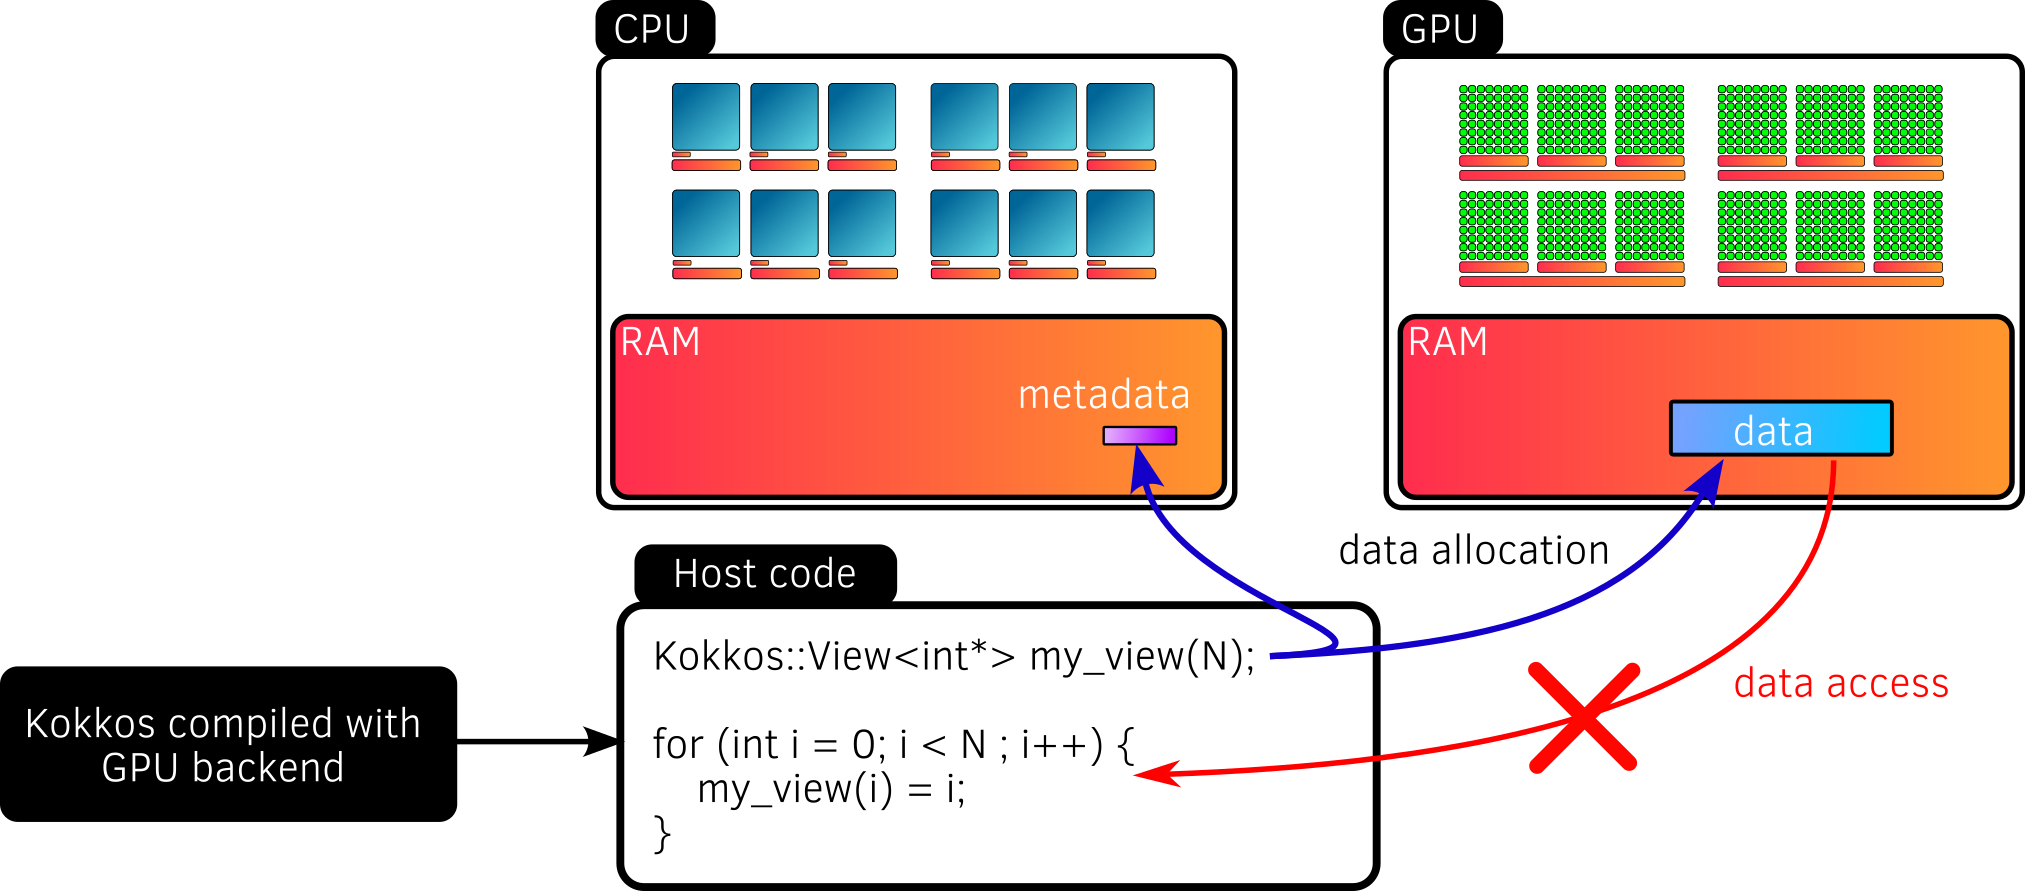
\includegraphics[width=\textwidth]{../../images/device_memory_access.png}
\end{center}

\end{frame}

% _____________________________________________________________________________

\begin{frame}[fragile]
    \frametitle{Understand the notion of memory space}

A template argument \highlight{MemorySpace} can be used to specify the memory space when creating a view

\begin{minted}[texcomments]{C++}
Kokkos::View<int**, MemorySpace> my_matrix("matrix", Nx, Ny);
\end{minted}

\begin{itemize}
    \item \texttt{Kokkos::HostSpace}: Host memory space
\end{itemize}

\begin{alertblock}{}
    \begin{itemize}
    \item Beginners should not explicitly define the memory space
    \item Using a vendor-specific memory space breaks the portability of the code
    \end{itemize}
\end{alertblock}

\end{frame}

% _____________________________________________________________________________

\begin{frame}[fragile]
    \frametitle{Mirror Views presentation}

\begin{itemize}
    \item \textbf{Solution:} we need linked host and device view to access the data on both sides
    \item Kokkos provides the notion of \textbf{mirror views}
    \item A mirror view is a view that is a copy of another view but in a different memory space
    \item There is a specific function to create a mirror view called \texttt{create\_mirror}
    \item It can be used to create a host mirror of a device view
\end{itemize}

\begin{minted}[texcomments]{C++}
Kokkos::View<int**> device_matrix("device_matrix", Nx, Ny);
Kokkos::View<int**>::HostMirror host_matrix = 
    Kokkos::create_mirror(device_matrix);
\end{minted}

\begin{itemize}
\item A mirror view automatically inherits the properties of the original view (extent, layout, etc)
\end{itemize}

\end{frame}

% _____________________________________________________________________________

\begin{frame}[fragile]
    \frametitle{Undestanding mirror View with a device View}

\begin{center}
    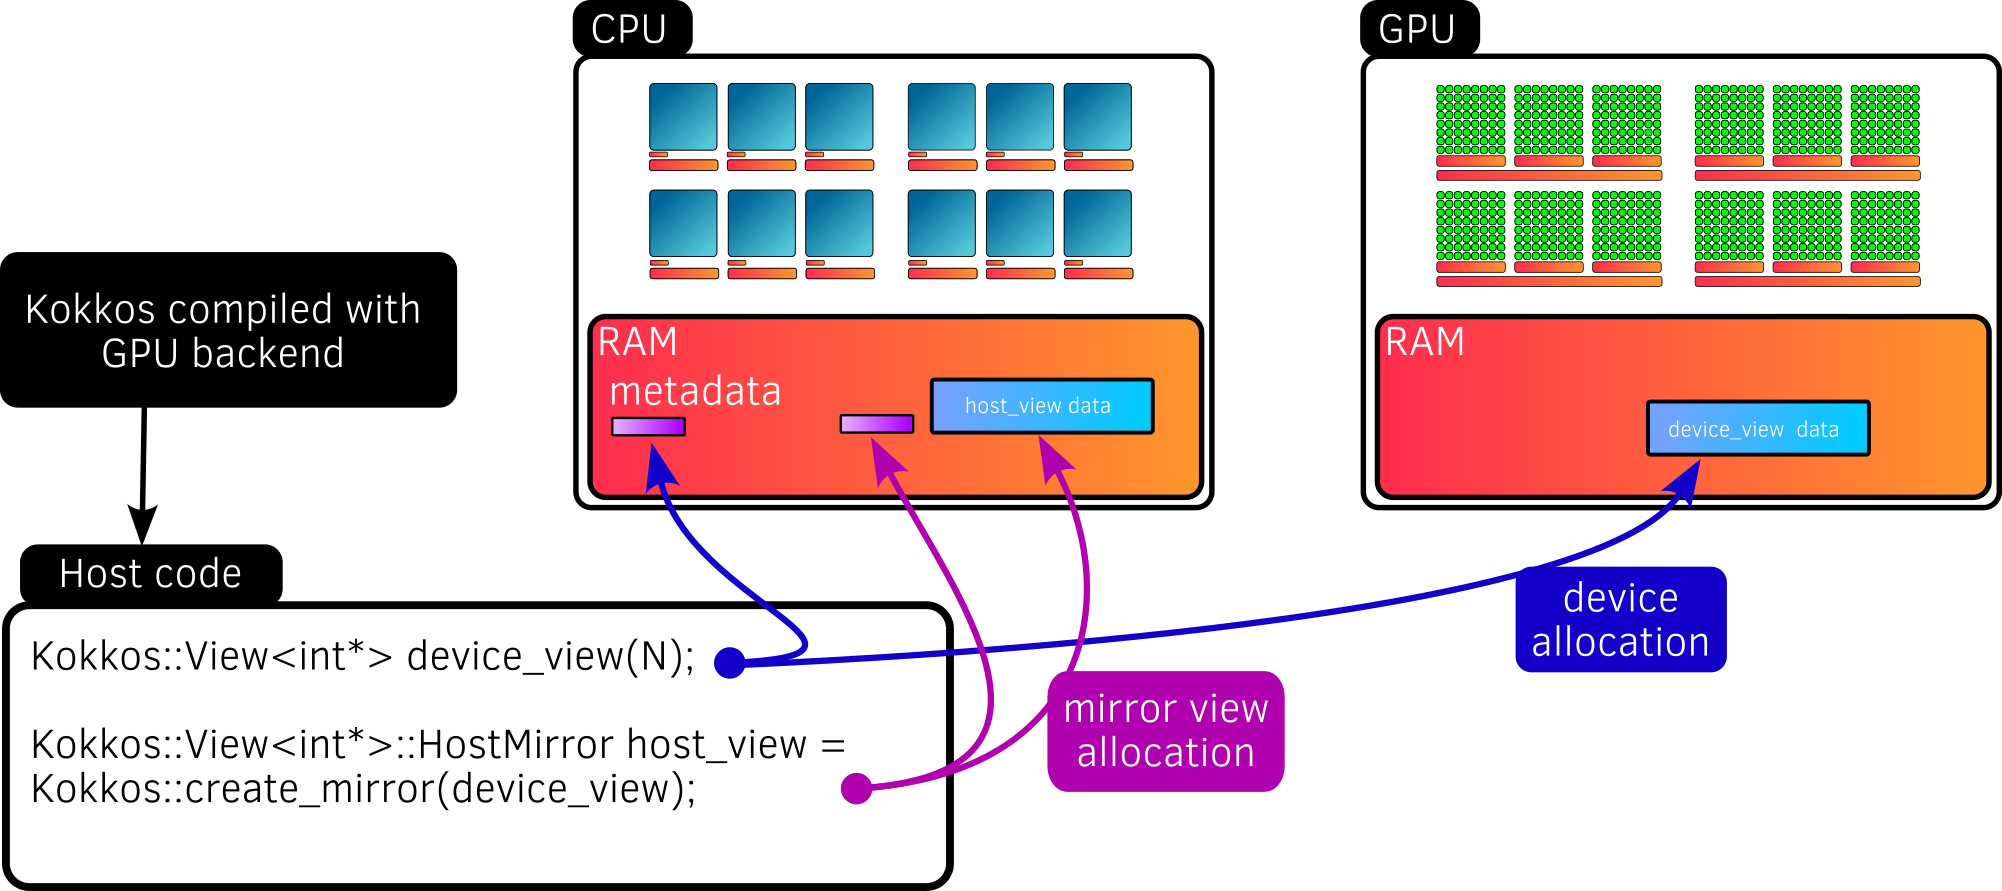
\includegraphics[width=\textwidth]{../../images/device_mirror_view.png}
\end{center}

\end{frame}

% _____________________________________________________________________________

\begin{frame}[fragile]
    \frametitle{Views and mirror Views in the host memory space}

\begin{itemize}
\item For portability reason, we use the mirror view whether we compile with a CPU or GPU backend
\item With a CPU backend only, the mirror view lives in the same memory space as the original view
\item \textbf{Problem:} the \texttt{create\_mirror} function always create a view with allocated memory (memory duplication)
\end{itemize}

\begin{center}
    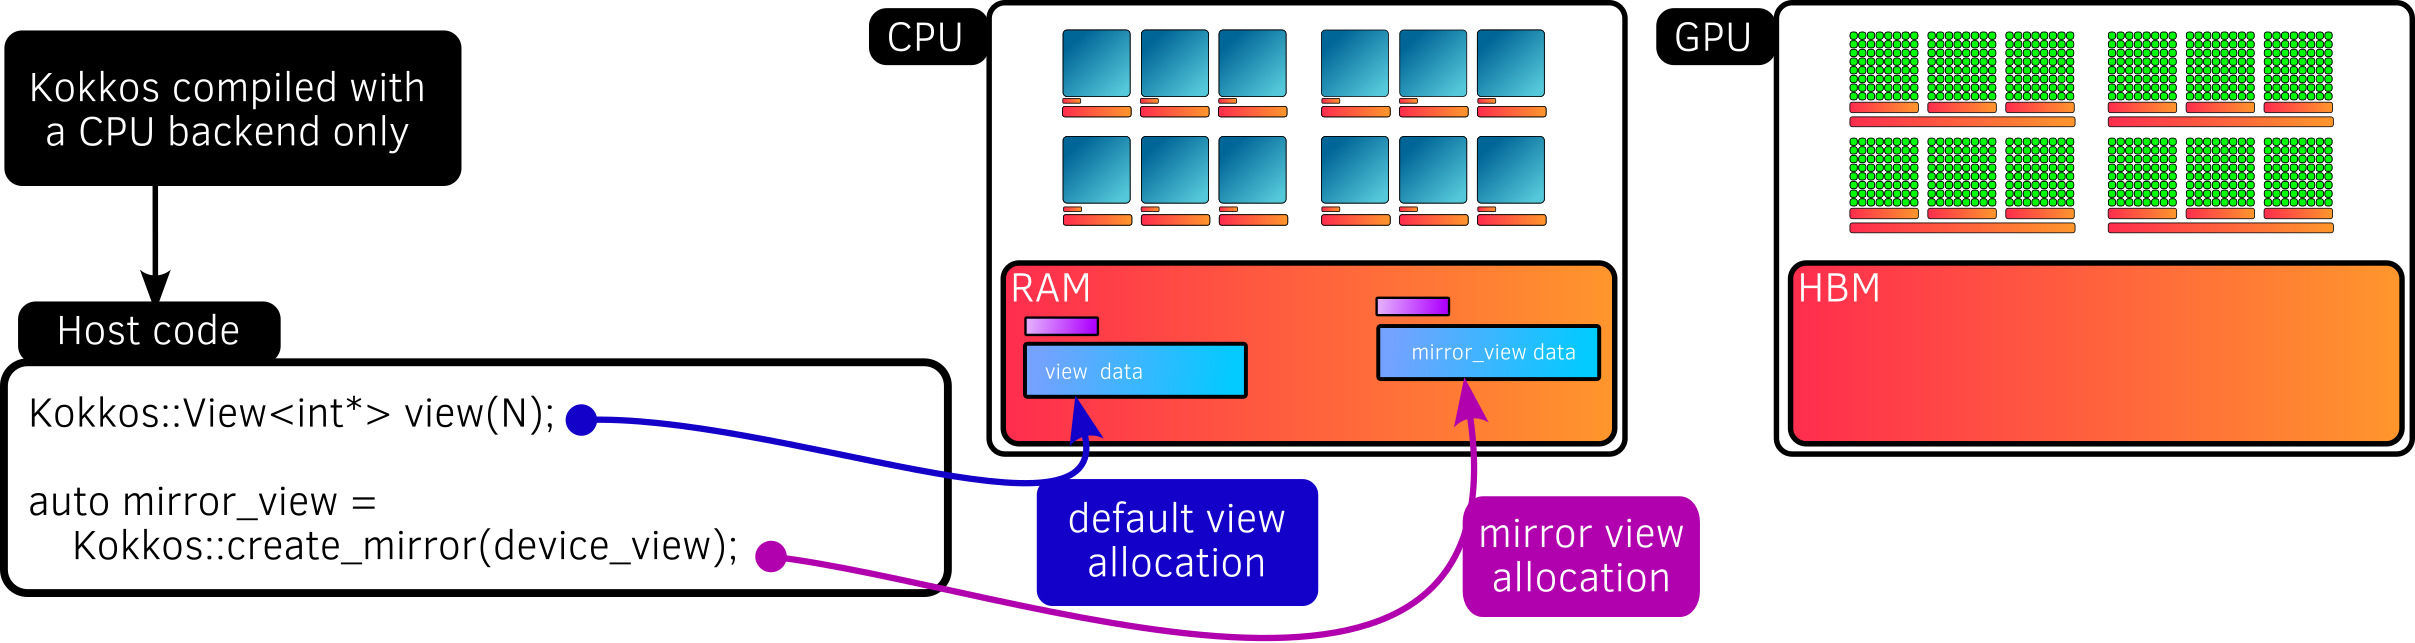
\includegraphics[width=0.9\textwidth]{../../images/host_mirror_view.png}
\end{center}

\end{frame}


% _____________________________________________________________________________

\begin{frame}[fragile]
    \frametitle{Views and mirror Views in the host memory space}

\begin{itemize}
    \item \textbf{Solution:} The function \texttt{create\_mirror\_view} can be used to create a mirror view without allocating memory if the mirror view lives in the same memory space as the original view
    \item The new view is a shallow copy of the original view (point to the same data)
\end{itemize}

\begin{center}
    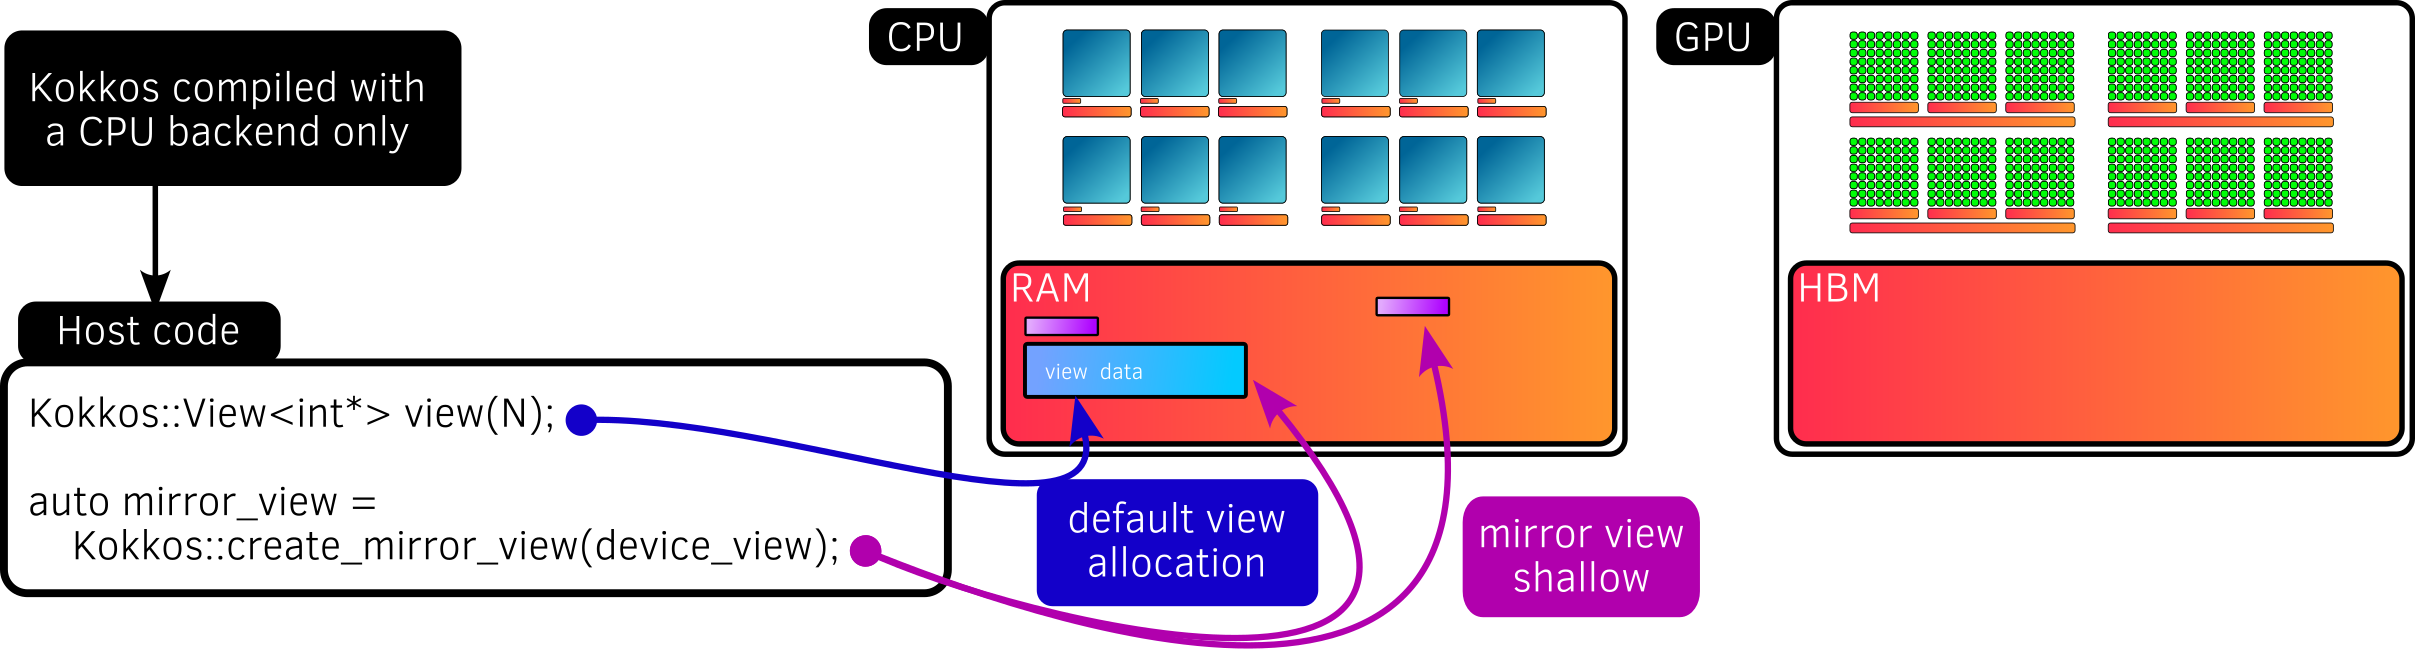
\includegraphics[width=0.9\textwidth]{../../images/host_create_mirror_view.png}
\end{center}

\end{frame}

% _____________________________________________________________________________

\begin{frame}[fragile]
    \frametitle{Deep copy function to exchange data between memory spaces}

\begin{itemize}
    \item Kokkos provides a function \texttt{deep\_copy} to copy data between views in different memory spaces
    \item Views must have the same layout and extent
    \item The function is used to copy data from the source view to the destination view
\end{itemize}

\begin{minted}[texcomments]{C++}
    Kokkos::deep_copy(destination, source);
\end{minted}

\begin{itemize}
    \item If the dest view is a shallow copy of the source view (\texttt{create\_mirror\_view} on Host for instance), the function does nothing (portability)
\end{itemize}
\end{frame}

% _____________________________________________________________________________

\begin{frame}[fragile]
    \frametitle{Deep copy example between Host and Device}

Example of deep copy between a device view and a host mirror view:

\begin{minted}[texcomments]{C++}
Kokkos::View<int**> device_matrix("device_matrix", Nx, Ny);

Kokkos::View<int**>::HostMirror host_matrix = 
    Kokkos::create_mirror(device_matrix);

Kokkos::deep_copy(device_matrix, host_matrix);
\end{minted}
\end{frame}

% _____________________________________________________________________________

\begin{frame}[fragile]
    \frametitle{Deep copy function to exchange data between memory spaces}

    \begin{center}
        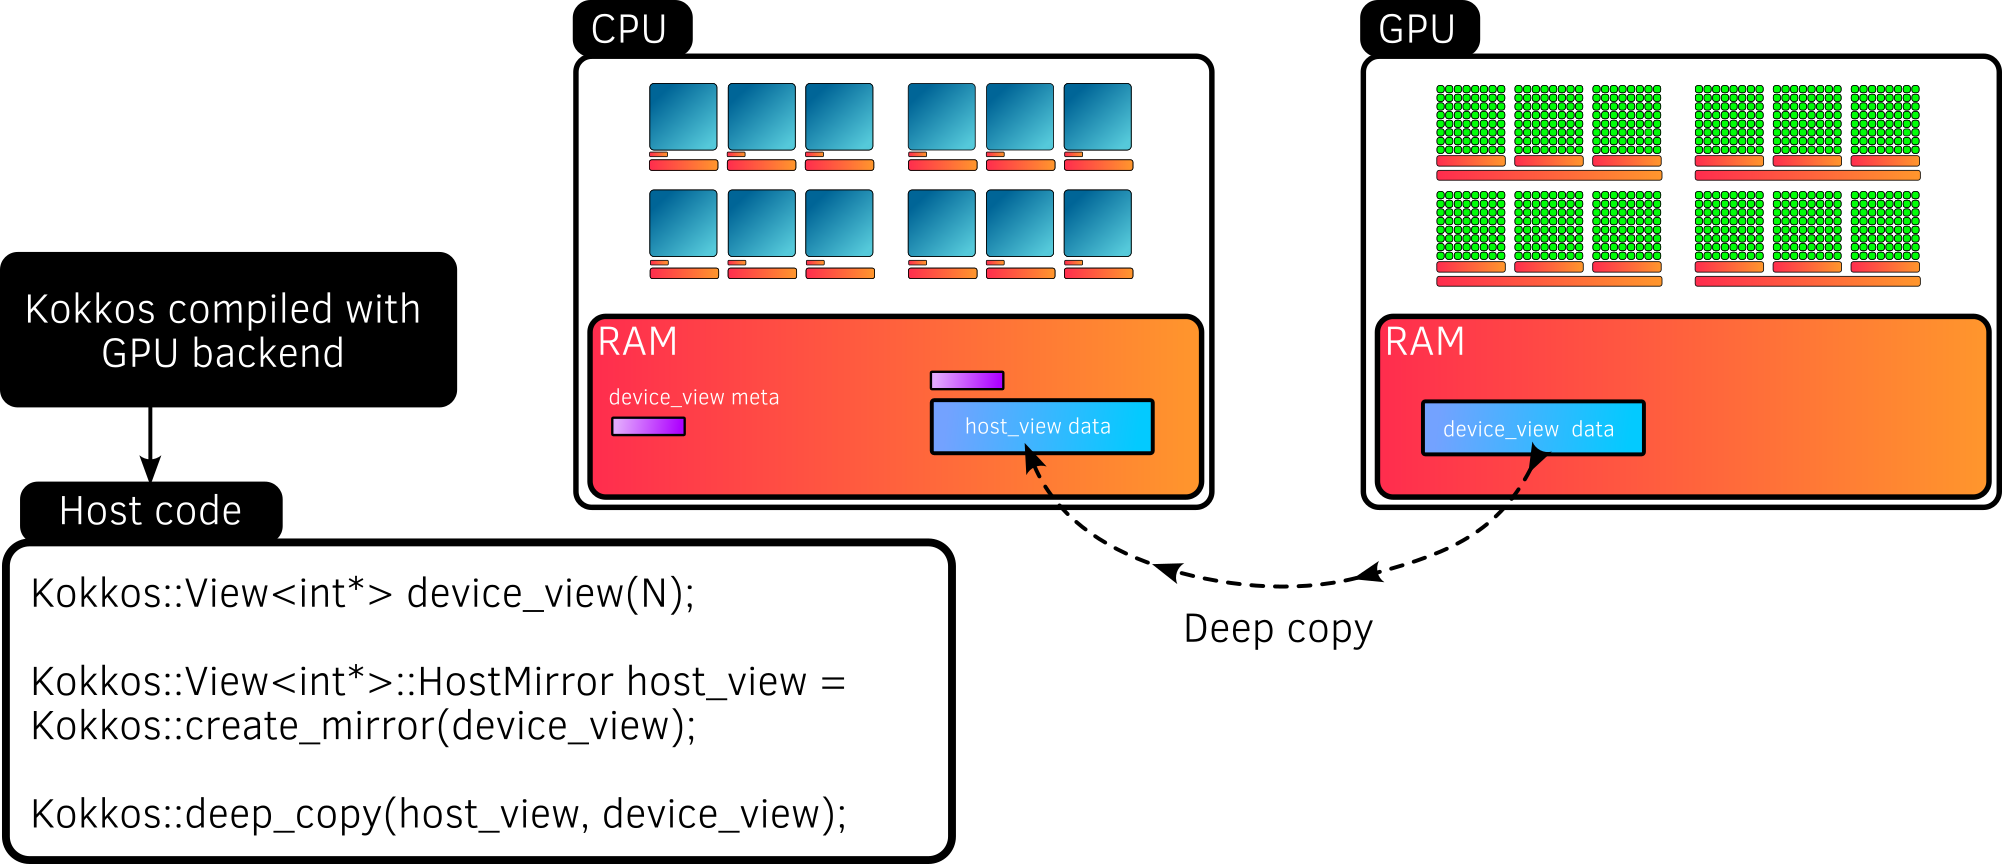
\includegraphics[width=0.9\textwidth]{../../images/device_host_deep_copy.png}
    \end{center}

\end{frame}

% _____________________________________________________________________________

\begin{frame}[fragile]
    \frametitle{Exercise 4: Mirror Views and deep copy} 

    \begin{center}
    
\includegraphics[width=0.4\textwidth]{../../images/sleeping_otter.png}
    \end{center}

    Goal of this exercise:

    \begin{itemize}
        \item Create and manage a mirror view
        \item Use the deep copy function
    \end{itemize}

    \begin{block}{}
        Go to the exercise \href{https://github.com/CExA-project/cexa-kokkos-tutorials/tree/main/exercises/04_deep_copy}{04\_deep\_copy} and follow the instructions in the README file
    \end{block}

\end{frame}

% _____________________________________________________________________________

\subsection[Data container]{Parallel loops}

% \begin{frame}[fragile]
%     \begin{center}
%     \Huge Basic concepts of Kokkos \\
%     \normalsize
%     Parallel loops
%     \end{center}
% \end{frame}

% _____________________________________________________________________________

\begin{frame}[fragile]
    \frametitle{Kokkos uses the concept of data parallelism as OpenMP} 


\begin{minted}[texcomments]{C++}
for (int i = 0; i < N; i++) {
    A(i) = B(i) + C(i)*D(i);
}
\end{minted}

\begin{itemize}
    \item \textcolor{gray}{\texttt{for}} is the loop pattern (for, reduction, scan, graph)
    \item \textcolor{gray}{\texttt{int i = 0; i < N; i++}} is the execution policy
    \item \textcolor{gray}{\texttt{A(i) = B(i) + C(i)*D(i)}} is the kernel
\end{itemize}

\end{frame}

% _____________________________________________________________________________

\begin{frame}[fragile]
    \frametitle{Simple parallel loop with Kokkos and OpenMP} 

FMA addition using a parallel loop:
\begin{itemize}
\item Kokkos version:
\end{itemize}

\small
\begin{minted}{C++}
Kokkos::parallel_for("my_loop", N, 
KOKKOS_LAMBDA(int i) {
    A(i) = B(i) + C(i)*D(i);
});
\end{minted}

\normalsize
\begin{itemize}
\item OpenMP version:
\end{itemize}
    
\small
\begin{minted}{C++}
#pragma omp parallel for
for (int i = 0; i < N; i++) {
    A(i) = B(i) + C(i)*D(i);
});
\end{minted}
\end{frame}

% _____________________________________________________________________________

\begin{frame}[fragile]
    \frametitle{Simple parallel loop with Kokkos explained} 

\normalsize
\begin{itemize}
    \item \textcolor{gray}{\texttt{Kokkos::parallel\_for}} is the loop pattern 
    \item \textcolor{gray}{\texttt{N}} and \texttt{int i} is the execution policy (can't be simpler)
    \item \textcolor{gray}{\texttt{KOKKOS\_LAMBDA(int i) \{ A(i) = B(i) + C(i)*D(i) \} }} is the kernel
\end{itemize}

\small
\begin{minted}{C++}
Kokkos::parallel_for("my_loop", N, 
KOKKOS_LAMBDA(int i) {
    A(i) = B(i) + C(i)*D(i);
});
\end{minted}

\normalsize
\begin{itemize}
    \item The previous OpenMP version only works on CPUs (need \texttt{target} directive for GPUs)
    \item The same Kokkos version works on CPUs and GPUs depending on the compile backend
\end{itemize}


\end{frame}

% _____________________________________________________________________________

\begin{frame}[fragile]
    \frametitle{Notion of C++ Lambda} 

\begin{itemize}
    \item A lambda is a C++ anonymous function
    \item \texttt{KOKKOS\_LAMBDA} is a macro that creates a lambda function with the correct signature for you
    \item For beginners, no need to Understand C++ lambda to use Kokkos
\end{itemize}

\small
\begin{minted}{C++}
Kokkos::parallel_for("my_loop", N, 
KOKKOS_LAMBDA(int i) {
    A(i) = B(i) + C(i)*D(i);
});
\end{minted}

\end{frame}

% _____________________________________________________________________________

\begin{frame}[fragile]
    \frametitle{Where is my parallel loop executed?}

\begin{itemize}
    \item Where the loop is executed is called the \textcolor{orange}{\textbf{execution space}}
    \item If Kokkos is compiled with a GPU backend, the loop is executed on GPU by default
    \item Else, the loop is executed on the CPU
    \item Non-kokkos C++ code is always executed on the Host
    \item Kokkos loops can have a name for debugging purpose
\end{itemize}

\end{frame}

% _____________________________________________________________________________

\begin{frame}[fragile]
    \frametitle{Asynchronous execution} 

\begin{itemize}
    \item Parallel loops are executed asynchronously, this mean that the loop is launched and the program continues
    \item Asynchronicity is a complex concept for beginners, not the subject of this introduction
\end{itemize}

\small
\begin{minted}{C++}
// Kokkos parallel loop
Kokkos::parallel_for("my_loop", N, KOKKOS_LAMBDA(int i) {...});

// Host code executed during the parallel loop 
// if Kokkos is compiled with a GPU backend
for (int i = 0; i < N; i++) { ... }
\end{minted}

\normalsize


\begin{itemize}
    \item If Kokkos uses a GPU backend, the parallel loop is executed asynchronously on the GPU
    \item \textbf{Problem:} what if I need the results of the parallel loop in the host code?
\end{itemize}

\end{frame}

% _____________________________________________________________________________

\begin{frame}[fragile]
    \frametitle{Fence} 

\begin{itemize}
    \item \textbf{Solution:} To make sure that the loop is finished, a \highlight{fence} function can be used (equivalent of an OpenMP barrier or a MPI wait)
\end{itemize}

\begin{minted}{C++}
void Kokkos::fence(const std::string& label);
\end{minted}

Example: the \texttt{fence} function ensures that the Kokkos parallel loop is finished before the host code starts:

\small
\begin{minted}{C++}
Kokkos::parallel_for("my_loop", N, KOKKOS_LAMBDA(int i) {...});

Kokkos::fence("my_fence");

for (int i = 0; i < N; i++) { ... }
\end{minted}

\end{frame}

% _____________________________________________________________________________

\begin{frame}[fragile]
    \frametitle{Exercise 5: My first parallel loop} 

    \begin{center}
    
\includegraphics[width=0.4\textwidth]{../../images/sleeping_otter.png}
    \end{center}

    Goal of this exercise:

    \begin{itemize}
        \item Write a simple parallel loop
    \end{itemize}

    \begin{block}{}
        Go to the exercise \href{https://github.com/CExA-project/cexa-kokkos-tutorials/tree/main/exercises/05_parallel_loop}{05\_parallel\_loop} and follow the instructions in the README file
    \end{block}

\end{frame}

% _____________________________________________________________________________

\subsection[Extended loop policy]{How to extent the loop policy}

% _____________________________________________________________________________

\begin{frame}[fragile]
    \frametitle{How to extent the loop policy ?}

\begin{itemize}
    \item Kokkos provides a way to tune the execution policy via the \highlight{RangePolicy} structure
\end{itemize}

\small
\begin{minted}{C++}
Kokkos::RangePolicy<ExecutionSpace> policy(start_index, end_index);
\end{minted}

\begin{itemize}
    \item \texttt{ExecutionSpace} is an optional template parameter that specifies the execution space, by default the execution space is \texttt{DefaultExecutionSpace}.
    \item \texttt{start\_index} and \texttt{end\_index} are the beginning and the end of the loop
\end{itemize}

\small
\begin{minted}{C++}
Kokkos::parallel_for("my_loop", 
    Kokkos::RangePolicy<ExecutionSpace>(start_index, end_index),
    KOKKOS_LAMBDA(int i) { ... });
\end{minted}

\end{frame}

% _____________________________________________________________________________

\begin{frame}[fragile]
    \frametitle{How to extent the loop policy ?}

The following parallel loops are therefore equivalent:

\small
\begin{minted}{C++}
// Short version
Kokkos::parallel_for("my_loop", 
    N,
    KOKKOS_LAMBDA(int i) { ... });
\end{minted}

\begin{minted}{C++}
// explicitly specify the execution policy
Kokkos::parallel_for("my_loop", 
    Kokkos::RangePolicy<Kokkos::DefaultExecutionSpace>(0, N),
    KOKKOS_LAMBDA(int i) { ... });
\end{minted}

\end{frame}

% _____________________________________________________________________________

\begin{frame}[fragile]
    \frametitle{Execution Space}

By specifying the execution space, you can control where the loop is executed.
This is the way to decide if a Kokkos parallel loop is executed on the CPU or the GPU.

\begin{itemize}
    \item \highlight{Kokkos::DefaultExecutionSpace} is the default execution space: if Kokkos is compiled with a GPU backend, the default execution space is the corresponding GPU execution space, else the default execution space is the Host execution space
    \item \highlight{Kokkos::DefaultHostExecutionSpace} is the default Host execution space and refers to the CPU backend used to compile Kokkos
    \item Other execution spaces are not the subject of this introduction
    \item This way of doing ensures that the code is portable
\end{itemize}

\end{frame}

% _____________________________________________________________________________

\begin{frame}[fragile]
    \frametitle{Default execution space summary}

\begin{center}
    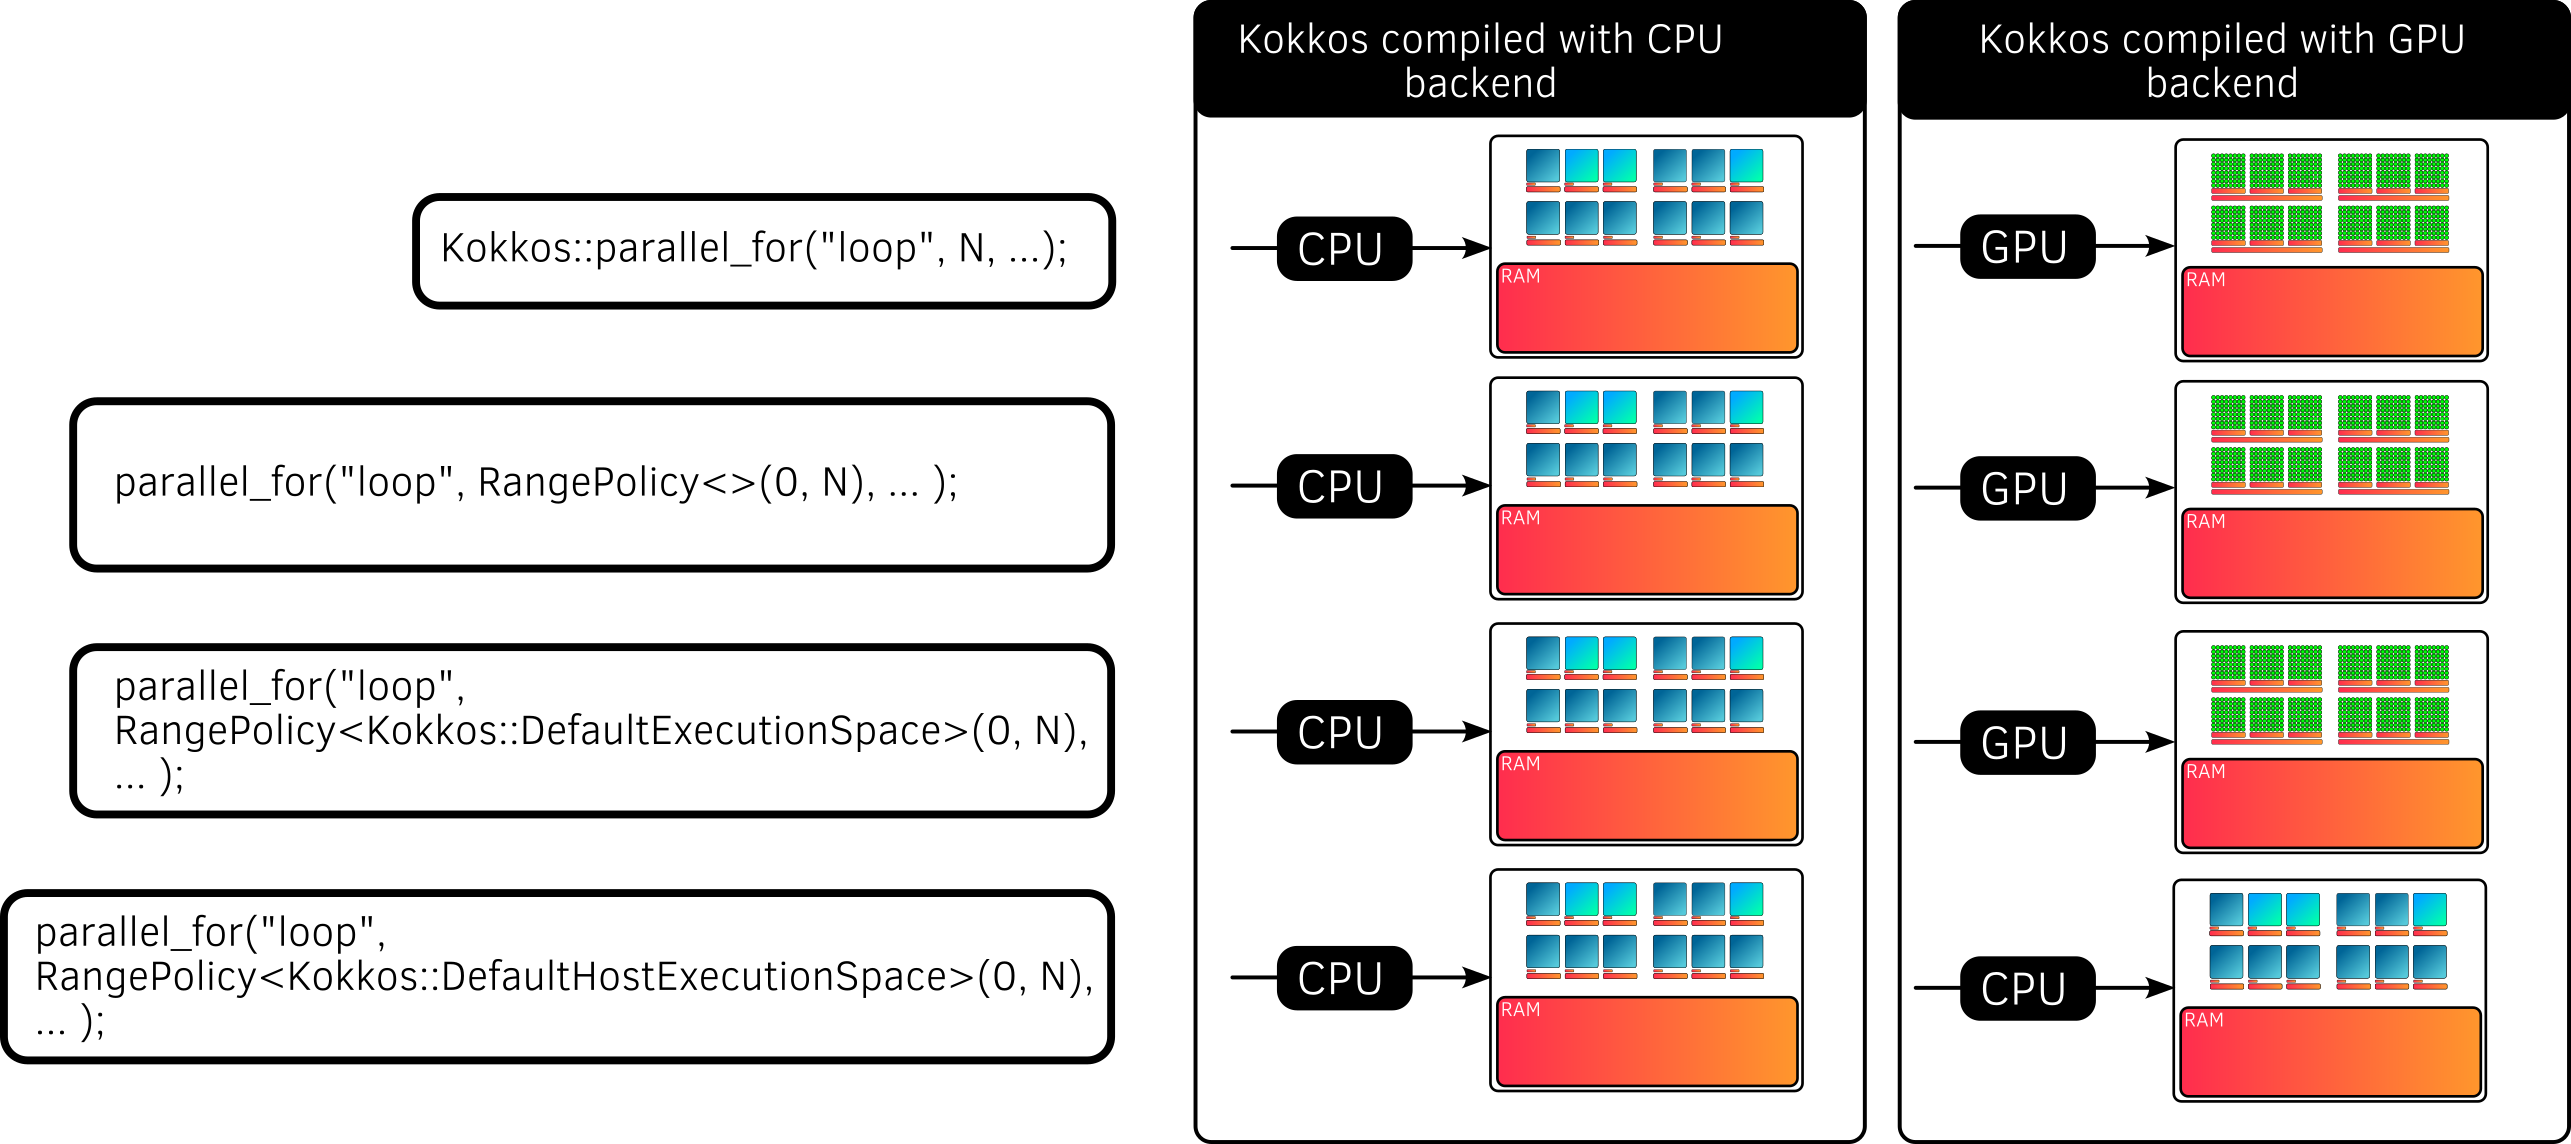
\includegraphics[width=\textwidth]{../../images/default_execution_space.png}
\end{center}

\end{frame}

% _____________________________________________________________________________

\begin{frame}[fragile]
    \frametitle{Relation between execution space and memory space}


The memory space associated with an execution space can be retrieved using the \highlight{memory\_space} attribute

\footnotesize
\begin{minted}{C++}
using DefaultMemorySpace = DefaultExecutionSpace::memory_space;
using DefaultHostMemorySpace = DefaultHostExecutionSpace::memory_space;
\end{minted}

\normalsize
By definition:
\begin{itemize}
    \item \texttt{HostSpace} and \texttt{DefaultHostExecutionSpace::memory\_space} are the same
    \item \texttt{SharedSpace} and \texttt{DefaultExecutionSpace::memory\_space} are the same
\end{itemize}

\end{frame}

% _____________________________________________________________________________

\begin{frame}[fragile]
    \frametitle{Nested parallel loops}

\begin{minted}{C++}

Kokkos::View<int**> my_matrix("matrix", Nx, Ny);

for (int i = 0; i < Nx; i++) {
    for (int j = 0; j < Ny; j++) {
        my_matrix(i,j) = i + j;
    }
}
\end{minted}

\end{frame}

% _____________________________________________________________________________

\begin{frame}[fragile]
    \frametitle{Nested parallel loops}

\begin{itemize}
    \item Kokkos allows nested parallel loops using the \highlight{MDRangePolicy} structure
    \item Somehow similar to the \texttt{collapse} directive in OpenMP
    \item Extension of the \texttt{RangePolicy} structure
    \item Addition of the Rank template parameter that specifies the number of dimensions
\end{itemize}

\footnotesize
\begin{minted}{C++}
Kokkos::MDRangePolicy<ExecutionSpace, 
                      Kokkos::Rank<2>> policy({start_index_0, start_index_1}, 
                                              {end_index_0, end_index_1});
\end{minted}

\normalsize
\begin{itemize}
    \item In some conditions, nested parallel loops can be more efficient than a single parallel loop via internal tilling optimization
\end{itemize}

\end{frame}

% _____________________________________________________________________________

\begin{frame}[fragile]
    \frametitle{Nested parallel loops in practice}

\footnotesize
\begin{minted}{C++}

Kokkos::View<int**> my_matrix("matrix", Nx, Ny);

Kokkos::parallel_for("my_loop", 
    Kokkos::MDRangePolicy<ExecutionSpace, Kokkos::Rank<2>>({0, 0}, {Nx, Ny}),
    KOKKOS_LAMBDA(int i, int j) { 
        my_matrix(i,j) = i + j;
    }
);
\end{minted}
\end{frame}

% _____________________________________________________________________________

\subsection[Parallel reduction]{Parallel reduction}

% _____________________________________________________________________________

\begin{frame}[fragile]
    \frametitle{Parallel reduction}

\begin{itemize}
\item Parallel reduction is the second loop pattern provided by Kokkos: \highlight{Kokkos::parallel\_reduce}
\item It is often used to compute a single value from an array (sum, max, min, etc.)
\item It works like the \texttt{parallel\_for} loop pattern but with an additional argument: the reducer operation to perform \highlight{Kokkos::Reducer\_op<type>}
\item \texttt{KOKKOS\_LAMBDA} also has an additional argument: a reference to the local result
\end{itemize}

\footnotesize
\begin{minted}{C++}
// No need to initialize the variable, it will be
// done by the parallel_reduce call
double result;

Kokkos::parallel_reduce("my_reduction", N,
KOKKOS_LAMBDA(int i, double& local_result) {
    // Reduction operation ...
}, Kokkos::Reducer_op<type>(result));
\end{minted}

\end{frame}

% _____________________________________________________________________________

\begin{frame}[fragile]
    \frametitle{Parallel reduction explained}

\begin{itemize}
    \item As for the \texttt{parallel\_for} loop pattern, where the loop is executed depends on the execution space and the compiled backends
    \item Reduction is always optimized for the selected execution space
    \item Kokkos provides reducers (\texttt{Reducer\_op}) for the most common operations:
    \begin{itemize}
        \item \texttt{Kokkos::Sum}: Sum of the elements
        \item \texttt{Kokkos::Max}: and \texttt{Kokkos::Min}: Maximum and minimum element
        \item \texttt{Kokkos::Prod}: Product of the elements
        \item \texttt{Kokkos::MaxLoc} and \texttt{Kokkos::MinLoc}: Maximum and minimum element with their index
        \item and mores
    \end{itemize}  
    \item You can also create your own reducer but this is not the subject of this introduction
\end{itemize}

\begin{block}{}
    Build-in reducers: \href{https://kokkos.org/kokkos-core-wiki/ProgrammingGuide/Custom-Reductions-Built-In-Reducers.html}{https://kokkos.org/kokkos-core-wiki/ProgrammingGuide/Custom-Reductions-Built-In-Reducers.html}
\end{block}

\end{frame}

% _____________________________________________________________________________

\begin{frame}[fragile]
    \frametitle{Sum reduction example}

Sum of an array using a parallel reduction:

\footnotesize
\begin{minted}{C++}
double result;
Kokkos::View<double*> A("A", N);
// ... Fill vector A with data ...
Kokkos::parallel_reduce("my_reduction", N,
KOKKOS_LAMBDA(int i, double& local_result) {
    local_result += A(i);
}, Kokkos::Sum<double>(result));
\end{minted}

\normalsize
Can be even shorter in this case:

\footnotesize
\begin{minted}{C++}
Kokkos::parallel_reduce("my_reduction", N,
KOKKOS_LAMBDA(int i, double& local_result) {
    local_result += A(i);
}, result);
\end{minted}

\end{frame}

% _____________________________________________________________________________

\begin{frame}[fragile]
    \frametitle{Max reduction example}

Max of an array using a parallel reduction:

\footnotesize
\begin{minted}{C++}
double max_value;

Kokkos::View<double*> A("A", N);
// ... Fill vector A with data ...
Kokkos::parallel_reduce("my_reduction", N,
KOKKOS_LAMBDA(int i, double& local_max_value) {
    if (A(i) > local_max_value) {
        local_max_value = A(i);
    }
}, Kokkos::Max<double>(max_value));
\end{minted}

\end{frame}

% _____________________________________________________________________________

\begin{frame}[fragile]
    \frametitle{Min and index reduction example}

Min and index of an array using a parallel reduction:

\footnotesize
\begin{minted}{C++}
Kokkos::View<double*> A("A", N);
// ... Fill vector A with data ...

// Use a structure containing val and loc variables
typedef Kokkos::MinLoc<double,int>::value_type minloc_type;
minloc_type minloc;

Kokkos::parallel_reduce( "MinLocReduce", N,
KOKKOS_LAMBDA (int i, minloc_type& lminloc) {
    if( A(i) < lminloc.val ) {
        lminloc.val = A(i);
        lminloc.loc = i;
    }
}, Kokkos::MinLoc<double,int>(minloc));
\end{minted}

\end{frame}

% _____________________________________________________________________________

\begin{frame}[fragile]
    \frametitle{Exercise 6: Parallel Reduction} 

    \begin{center}
    
\includegraphics[width=0.4\textwidth]{../../images/sleeping_otter.png}
    \end{center}

    Goal of this exercise:

    \begin{itemize}
        \item Perform a parallel reduction
    \end{itemize}

    \begin{block}{}
        Go to the exercise \href{https://github.com/CExA-project/cexa-kokkos-tutorials/tree/main/exercises/06_parallel_reduce}{06\_parallel\_reduce} and follow the instructions in the README file
    \end{block}

\end{frame}

% _____________________________________________________________________________

\section[Conclusion]{Conclusion}

% _____________________________________________________________________________

\begin{frame}[fragile]
    \frametitle{Conclusion}

Congratulation, you have learned the basics of Kokkos:

\begin{itemize}
    \item How to compile Kokkos
    \item How to create and manage a simple View
    \item How to use mirror views and deep copy
    \item How to write a parallel loop
    \item How to extend the loop policy
    \item How to use nested parallel loops
    \item How to write a parallel reduction
\end{itemize}

\end{frame}

\end{document}
